%==============================================================
% Computer Graphics Laboratory Project Report - Neon Genesis
% Dewan Salman Rahman Zisan (2107015)
% Khulna University of Engineering & Technology
%==============================================================

\documentclass[12pt, a4paper]{report}

%--------------------------------------------------------------
% PACKAGES
%--------------------------------------------------------------
\usepackage[T1]{fontenc}
\usepackage{mathptmx}           % Times Roman font
\usepackage[utf8]{inputenc}
\usepackage{geometry}
\usepackage{setspace}
\usepackage{titlesec}
\usepackage{tocloft}
\usepackage{graphicx}
\usepackage{caption}
\usepackage{fancyhdr}
\usepackage{emptypage}
\usepackage{indentfirst}
\usepackage{ragged2e}
\usepackage{booktabs}
\usepackage{array}
\usepackage{amsmath}
\usepackage{hyperref}
\usepackage{float}
\usepackage{longtable}
\usepackage{etoolbox}
\usepackage{placeins}
\usepackage{tikz}
\usetikzlibrary{positioning, fit, backgrounds, arrows.meta}

%--------------------------------------------------------------
% LAYOUT
% - every chapter starts on a new page (the report class default)
% - tables and figures use single line spacing
% - headings use single-spaced lines so they do not open large gaps
%--------------------------------------------------------------
\AtBeginEnvironment{table}{\setstretch{1.0}}
\AtBeginEnvironment{figure}{\setstretch{1.0}}
\setlength{\textfloatsep}{10pt plus 2pt minus 2pt}
\setlength{\floatsep}{8pt plus 2pt minus 2pt}
\setlength{\intextsep}{8pt plus 2pt minus 2pt}
\renewcommand{\topfraction}{0.85}
\renewcommand{\textfraction}{0.10}
\renewcommand{\floatpagefraction}{0.75}

%--------------------------------------------------------------
% BLANK LINE HELPER
%--------------------------------------------------------------
\newcommand{\blanklines}[1]{\vspace{#1\dimexpr 18pt\relax}}

%--------------------------------------------------------------
% PAGE GEOMETRY
%--------------------------------------------------------------
\geometry{
  a4paper,
  top=1.2in,
  bottom=1.0in,
  left=1.2in,
  right=1.0in,
  headheight=14pt,
  headsep=0.2in,
  footskip=0.4in
}

%--------------------------------------------------------------
% LINE SPACING
%--------------------------------------------------------------
\setstretch{1.5}

%--------------------------------------------------------------
% PARAGRAPH SPACING
%--------------------------------------------------------------
\setlength{\parskip}{3pt}
\setlength{\parindent}{0pt}

%--------------------------------------------------------------
% HEADER / FOOTER
%--------------------------------------------------------------
\pagestyle{fancy}
\fancyhf{}
\fancyhead[C]{\fontsize{12}{14}\selectfont}
\fancyfoot[C]{\thepage}
\renewcommand{\headrulewidth}{0pt}
\renewcommand{\footrulewidth}{0pt}

\fancypagestyle{plain}{
  \fancyhf{}
  \fancyfoot[C]{\thepage}
  \renewcommand{\headrulewidth}{0pt}
  \renewcommand{\footrulewidth}{0pt}
}

%--------------------------------------------------------------
% CHAPTER STYLE
% Use Roman numerals (CHAPTER I, II, III ...) per template
%--------------------------------------------------------------
\renewcommand{\thechapter}{\Roman{chapter}}
\titleformat{\chapter}[block]
  {\fontsize{16}{20}\bfseries\centering\setstretch{1.0}}
  {CHAPTER \thechapter}
  {1em}
  {}
\titlespacing*{\chapter}{0pt}{0pt}{14pt}

%--------------------------------------------------------------
% SECTION STYLE
%--------------------------------------------------------------
\titleformat{\section}
  {\fontsize{14}{17}\bfseries\raggedright\setstretch{1.0}}
  {\thesection}
  {1em}
  {}
\titlespacing*{\section}{0pt}{10pt}{3pt}

%--------------------------------------------------------------
% SUBSECTION STYLE
%--------------------------------------------------------------
\titleformat{\subsection}
  {\fontsize{12}{15}\bfseries\raggedright\setstretch{1.0}}
  {\thesubsection}
  {1em}
  {}
\titlespacing*{\subsection}{0pt}{8pt}{2pt}

%--------------------------------------------------------------
% TABLE OF CONTENTS
%--------------------------------------------------------------
\renewcommand{\contentsname}{Contents}
\renewcommand{\cfttoctitlefont}{\fontsize{16}{24}\bfseries\hfill}
\renewcommand{\cftaftertoctitle}{\hfill}
\setlength{\cftbeforetoctitleskip}{0pt}
\setlength{\cftaftertoctitleskip}{36pt}

\renewcommand{\cftchapfont}{\bfseries\fontsize{12}{18}\selectfont}
\renewcommand{\cftchappagefont}{\bfseries\fontsize{12}{18}\selectfont}
\setlength{\cftbeforechapskip}{6pt}

% Add "CHAPTER" prefix in TOC so entries read
% "CHAPTER I    Introduction    1" instead of "1 Introduction"
\renewcommand{\cftchappresnum}{CHAPTER\ }
\renewcommand{\cftchapaftersnum}{\quad}
\settowidth{\cftchapnumwidth}{CHAPTER\ XII\quad}

\renewcommand{\cftsecfont}{\fontsize{12}{18}\selectfont}
\renewcommand{\cftsecpagefont}{\fontsize{12}{18}\selectfont}
\setlength{\cftsecindent}{0.5in}
\setlength{\cftsubsecindent}{1.0in}

%--------------------------------------------------------------
% LIST OF TABLES
%--------------------------------------------------------------
\renewcommand{\listtablename}{List of Tables}
\renewcommand{\cftlottitlefont}{\fontsize{16}{24}\bfseries\hfill}
\renewcommand{\cftafterlottitle}{\hfill}
\setlength{\cftbeforelottitleskip}{0pt}
\setlength{\cftafterlottitleskip}{36pt}
\renewcommand{\cfttabfont}{\fontsize{12}{18}\selectfont}
\renewcommand{\cfttabpagefont}{\fontsize{12}{18}\selectfont}

%--------------------------------------------------------------
% LIST OF FIGURES
%--------------------------------------------------------------
\renewcommand{\listfigurename}{List of Figures}
\renewcommand{\cftloftitlefont}{\fontsize{16}{24}\bfseries\hfill}
\renewcommand{\cftafterloftitle}{\hfill}
\setlength{\cftbeforeloftitleskip}{0pt}
\setlength{\cftafterloftitleskip}{36pt}
\renewcommand{\cftfigfont}{\fontsize{12}{18}\selectfont}
\renewcommand{\cftfigpagefont}{\fontsize{12}{18}\selectfont}

%--------------------------------------------------------------
% FIGURE & TABLE CAPTION
%--------------------------------------------------------------
\captionsetup{
  font={rm,normalfont},
  labelfont=normalfont,
  textfont=normalfont,
  justification=centering,
  size=small,
  skip=6pt
}
\captionsetup[table]{position=above, skip=6pt}
\captionsetup[figure]{position=below, skip=6pt}

\renewcommand{\thefigure}{\arabic{chapter}.\arabic{figure}}
\renewcommand{\thetable}{\arabic{chapter}.\arabic{table}}

%--------------------------------------------------------------
% HYPERREF
%--------------------------------------------------------------
\hypersetup{
  colorlinks=false,
  pdfborder={0 0 0}
}

% Equation numbers as (3.1), matching figures and tables
\renewcommand{\theequation}{\arabic{chapter}.\arabic{equation}}

%==============================================================
% DOCUMENT BEGINS
%==============================================================
\begin{document}

%--------------------------------------------------------------
% COVER PAGE
%--------------------------------------------------------------
\thispagestyle{empty}
\begin{center}

  % University logo: figures/logo.png (or logo.png next to this file). If it
  % is missing, an empty space of the same size is left.
  \IfFileExists{figures/logo.png}{
\includegraphics[height=1.3in]{figures/logo.png}}{%
    \IfFileExists{logo.png}{\includegraphics[height=1.3in]{logo.png}}{\rule{0pt}{1.3in}}}

  \vspace{10pt}

  {\fontsize{14}{21}\selectfont CSE 4102: Computer Graphics and Image Processing Laboratory}

  {\fontsize{18}{27}\bfseries\scshape
    Neon Genesis: A Procedurally Generated \\
    Real-Time Cyberpunk City with \\
    Ray-Traced Shadows in OpenGL
  }

  \blanklines{2}

  {\fontsize{14}{21}\selectfont By}

  \blanklines{1}

  {\fontsize{14}{21}\bfseries Dewan Salman Rahman Zisan}\\[0pt]
  {\fontsize{14}{21}\selectfont Roll: 2107015}

  \blanklines{2}

  {\fontsize{13}{18}\bfseries Submitted to}

  \begin{spacing}{1.2}
  {\fontsize{12}{16}\selectfont
    \textbf{Md Tajmilur Rahman}\\
    Lecturer\\[6pt]
    \textbf{Md. Mubtashim Abrar Nihal}\\
    Lecturer\\[6pt]
    Department of Computer Science and Engineering\\
    Khulna University of Engineering \& Technology
  }
  \end{spacing}

  \vfill
  \begin{spacing}{1.2}
    {\fontsize{12}{14}\bfseries
      Department of Computer Science and Engineering\\
      Khulna University of Engineering \& Technology\\
      Khulna 9203, Bangladesh\\
      October, 2026
    }
  \end{spacing}

\end{center}

%--------------------------------------------------------------
% ABSTRACT (page i)
%--------------------------------------------------------------
\newpage
\pagenumbering{roman}
\setcounter{page}{1}
\thispagestyle{plain}
\addcontentsline{toc}{chapter}{Abstract}

\begin{center}
  {\fontsize{16}{24}\bfseries Abstract}
\end{center}

\blanklines{1}

\begin{justify}
  {\fontsize{12}{13.8}\selectfont
    Neon Genesis is a real-time OpenGL 3.3 application that renders a rainy cyberpunk city at night and lets the user fly through it, drive a car in it, and watch it change from sunset to night. A seeded generator builds a $4\times4$ block island city of 53 towers in five styles with neon, billboards, 80 street lamps, 25 signalised junctions and distant districts, and every moving element is driven by one global clock.

    The renderer implements four light types (ambient, directional, point and spot) under the Blinn--Phong reflection model, with three switchable shading modes: flat, Gouraud and Phong. On top of this rasterised pipeline it adds hybrid ray tracing: every pixel fires a shadow ray toward the sun or moon, accelerated by a uniform grid over the city blocks. Further effects are Fresnel planar reflections, HDR bloom with Reinhard tone mapping, fog, a procedural sky and procedural textures, plus a switchable detail layer of bump-mapped facades, puddles, light beams, car reflections, a moonlit sea and lens effects. AI traffic with signal rules, a drivable car, music and a camera tour complete the project. On an AMD Ryzen 5 5500U with integrated Vega~7 graphics the application runs at roughly 77--160 frames per second at $1280\times720$ with every effect enabled, and a dynamic-resolution controller keeps it above 45 FPS under load.
  }
\end{justify}

%--------------------------------------------------------------
% TABLE OF CONTENTS (chapters and sections, single spaced)
%--------------------------------------------------------------
\newpage
\thispagestyle{plain}
\setcounter{tocdepth}{1}
\begin{spacing}{1.0}
\tableofcontents
\end{spacing}

%--------------------------------------------------------------
% MAIN MATTER
%--------------------------------------------------------------
\clearpage
\pagenumbering{arabic}
\setcounter{page}{1}

%==============================================================
% CHAPTER I: Introduction
%==============================================================
\chapter{Introduction}

\section{Introduction}

\begin{justify}
  {\fontsize{12}{13.8}\selectfont
    The goal of this project was to build a complete real-time 3D scene that exercises the core topics of the computer graphics course, namely geometric transformation, lighting, shading, animation and user interaction, and then to go beyond them with ray tracing and modern post-processing. A neon cyberpunk city was chosen because its many lights, wet reflections and constant motion make every technique visible. The project started from the GLFW + GLAD + GLM starter code used in the laboratory and grew into a 7,131-line C++ program organised into ten source files.
  }
\end{justify}

\section{Problem Statement}

\begin{justify}
  {\fontsize{12}{13.8}\selectfont
    The problem addressed is: \textit{how to procedurally generate and render a large, animated, multi-light city with physically motivated lighting, shading, shadows and reflections in real time on an integrated GPU, while keeping every feature interactive and explainable.}
  }
\end{justify}

\section{Objectives}

\begin{justify}
  {\fontsize{12}{13.8}\selectfont
    \begin{enumerate}
      \item Generate a reproducible city procedurally from a single seed.
      \item Model every object from a small set of primitives using translation, rotation, scaling and hierarchical transformations.
      \item Implement ambient, directional, point and spot lights with the Blinn--Phong model, and flat, Gouraud and Phong shading.
      \item Animate traffic, rain, signals, signs and the time of day from one clock.
      \item Add ray-traced shadows, reflections, bloom, fog and a procedural sky.
      \item Provide rich keyboard and mouse interaction, including a drivable car.
      \item Keep the application above 60 FPS on integrated graphics.
    \end{enumerate}
  }
\end{justify}

\section{Scope}

\begin{justify}
  {\fontsize{12}{13.8}\selectfont
    Windows, OpenGL 3.3 Core, MinGW-w64 g++, GLFW, GLAD and GLM; audio and images use Windows MCI and GDI+. Hardware ray-tracing APIs are out of scope; ray tracing runs in the fragment shader.
  }
\end{justify}

\section{Unfamiliarity of the Problem/Topic/Solution}

\begin{justify}
  {\fontsize{12}{13.8}\selectfont
    Floating-point framebuffers, shader ray tracing with an acceleration structure, planar reflections, bump mapping without stored tangents, spline camera paths and traffic simulation all went beyond the laboratory exercises and were adapted from the references to an integrated GPU.
  }
\end{justify}

\section{Project Planning}

\begin{justify}
  {\fontsize{12}{13.8}\selectfont
    Work proceeded in seven stages, each ending in a runnable build: geometry and camera; lighting, shading and post-processing; buildings and cars; traffic and driving; island and water; dusk and ray tracing; detail effects.
  }
\end{justify}

\section{Applications of the Work}

\begin{justify}
  {\fontsize{12}{13.8}\selectfont
    The techniques used here are the same ones that drive video games, driving and flight simulators, architectural walk-throughs and city visualisation: procedural content, many-light rendering, hybrid ray tracing and traffic simulation. Because every effect can be switched on and off at run time, the program is also useful as a teaching tool, for example to show the difference between Gouraud and Phong shading, or a scene with and without ray-traced shadows, on the same frame. The seeded generator means a new city can be produced instantly for testing or demonstration.
  }
\end{justify}

\section{Organization of the Report}

\begin{justify}
  {\fontsize{12}{13.8}\selectfont
    Chapter 2 reviews related techniques, Chapter 3 the methodology, Chapter 4 the results, Chapters 5--6 impact and engineering problems, and Chapter 7 concludes.
  }
\end{justify}

%==============================================================
% CHAPTER II: Related Works
%==============================================================
\chapter{Related Works}

\section{Introduction}

\begin{justify}
  {\fontsize{12}{13.8}\selectfont
    The lighting model follows Phong [5] and its Blinn half-vector refinement [6]; Gouraud's per-vertex interpolation [7] is kept as an alternative shading mode. Ray tracing originates with Whitted [8]; the ray--box test is the slab method of Kay and Kajiya [9] and the grid traversal is the DDA of Amanatides and Woo [10]. Bump mapping follows Blinn [17]. Tone mapping follows Reinhard et al. [11], the reflection uses Schlick's Fresnel approximation [12], camera paths use Catmull--Rom splines [13] and the clouds use value noise in the spirit of Perlin [14]. The practical OpenGL structure (framebuffers, bloom, shader organisation) follows the LearnOpenGL tutorials [4].
  }
\end{justify}

\section{Related Systems}

\begin{justify}
  {\fontsize{12}{13.8}\selectfont
    Procedurally generated cities are an established topic: Parish and M\"uller's CityEngine grows road networks and buildings from rules [18], and games such as \textit{Cyberpunk 2077} and \textit{Ghostrunner} made the rainy neon city a familiar visual style, but they rely on large art teams and dedicated GPUs. Hardware ray-tracing APIs are not available on integrated graphics such as Vega~7, but a uniform grid traversed with a DDA [10] makes shader-based ray tracing fast enough. This project combines these ideas at laboratory scale: a seeded city like CityEngine, the neon look of the games, and hybrid ray-traced shadows computed in an ordinary OpenGL 3.3 fragment shader.
  }
\end{justify}

\begin{justify}
  {\fontsize{12}{13.8}\selectfont
    For lighting, many-light renderers usually use deferred or clustered shading to handle hundreds of lights. These need several large render targets, which are expensive on an integrated GPU, so this project uses a simpler forward renderer that ranks the lights by importance every frame and shades with the best 24. For the same reason, planar (mirror) reflection was preferred to screen-space reflection.
  }
\end{justify}

\section{Discussion}

\begin{justify}
  {\fontsize{12}{13.8}\selectfont
    Table 2.1 summarises the main choices. In every case the technique taught in the course or a long-established method was preferred over the newest one when the newer method would not run well on integrated graphics or would be harder to explain.
  }
\end{justify}

\begin{table}[!htbp]
  \caption{Technique Choices and Alternatives}
  \label{tab:2.1}
  \centering
  {\fontsize{10}{13}\selectfont
    \begin{tabular}{|p{1.0in}|p{1.45in}|p{1.3in}|p{1.65in}|}
      \hline
      \textbf{Effect} & \textbf{Chosen} & \textbf{Alternative} & \textbf{Reason} \\
      \hline
      Shadows & Ray-traced shadow rays with grid & Shadow mapping & No aliasing or bias tuning; earns ray-tracing credit; grid keeps it cheap \\
      \hline
      Reflections & Planar mirrored pass & Screen-space reflection & SSR fell below 30 FPS in tests and cannot reflect off-screen objects \\
      \hline
      Glow & Separable Gaussian bloom at half resolution & Full-resolution 2D blur & 18 instead of 81 samples per pixel, at a quarter of the pixels \\
      \hline
      Tone mapping & Reinhard + saturation & ACES filmic & ACES crushed dark walls to black \\
      \hline
    \end{tabular}
  }
\end{table}

\begin{justify}
  {\fontsize{12}{13.8}\selectfont
    Table 2.2 lists the source followed for each technique and where it is used in the project, so every implemented feature can be traced back to its reference.
  }
\end{justify}

\begin{table}[!htbp]
  \caption{Techniques, Their Sources and Where They Are Used}
  \label{tab:2.2}
  \centering
  {\fontsize{10}{12.5}\selectfont
    \begin{tabular}{|p{1.8in}|p{1.3in}|p{2.3in}|}
      \hline
      \textbf{Technique} & \textbf{Source} & \textbf{Used for} \\
      \hline
      Phong / Blinn--Phong reflection & [5], [6] & all lighting, every shading mode \\
      \hline
      Gouraud shading & [7] & per-vertex shading mode (key 2) \\
      \hline
      Ray tracing, slab test, grid DDA & [8], [9], [10] & sun and moon shadows (key H) \\
      \hline
      Fresnel (Schlick) & [12] & wet road, water, car paint \\
      \hline
      Bump mapping & [17] & facade relief, puddle ripples \\
      \hline
      Tone mapping & [11] & HDR to screen colours \\
      \hline
      Catmull--Rom spline & [13] & camera tour (key V) \\
      \hline
      Value noise / fBm & [14] & clouds, textures, puddle mask \\
      \hline
      Procedural city & [18] & seeded city layout and buildings \\
      \hline
      OpenGL structure, bloom & [1]--[4], [16] & framebuffers, shaders, post-processing \\
      \hline
    \end{tabular}
  }
\end{table}

\section{Conclusion}

\begin{justify}
  {\fontsize{12}{13.8}\selectfont
    The project builds on well-established methods rather than new research: the lighting and shading models taught in the course, classic ray-tracing algorithms and standard real-time post-processing. Its contribution is combining them in one interactive scene that runs on ordinary laptop hardware.
  }
\end{justify}

%==============================================================
% CHAPTER III: Methodology
%==============================================================
\chapter{Methodology}

\section{Detailed Methodology}

\subsection{System Architecture and Frame Pipeline}

\begin{justify}
  {\fontsize{12}{13.8}\selectfont
    The code is split by responsibility: \texttt{main.cpp} (window, input, frame loop, drawing), \texttt{shaders.h} (all GLSL), \texttt{mesh.h} (primitive and extruded meshes), \texttt{city.h} (procedural generation), \texttt{traffic.h} (traffic and player car), \texttt{raytrace.h} (ray-tracing data), \texttt{render.h} (framebuffers and bloom), \texttt{textures.h}, \texttt{images.h} and \texttt{music.h}. Figure 3.1 shows the per-frame pipeline.
  }
\end{justify}

\begin{figure}[!htbp]
  \centering
  \begin{tikzpicture}[
      node distance = 5mm and 4mm,
      box/.style  = {draw, rounded corners=2pt, align=center, font=\footnotesize,
                     minimum height=10mm, text width=21mm, fill=gray!8},
      post/.style = {box, fill=blue!6},
      arr/.style  = {-{Stealth[length=2mm]}, thick}]
    % row 1: update, light selection and the first scene passes
    \node[box]                 (upd)   {Update\\(one clock)};
    \node[box, right=of upd]   (lit)   {Select best\\24 lights};
    \node[box, right=of lit]   (sky)   {Sky\\(moon, clouds)};
    \node[box, right=of sky]   (ref)   {Mirrored city\\(reflection)};
    \node[box, right=of ref]   (wat)   {Road \& water\\(Fresnel blend)};
    % row 2: the rest of the scene, then post-processing back to the left
    \node[box, below=9mm of wat]  (city)  {City: Blinn--Phong\\+ RT shadows};
    \node[box, left=of city]      (rain)  {Rain, ripples,\\light beams};
    \node[post, below=9mm of lit] (bloom) {Bloom +\\lens streaks};
    \node[post, below=9mm of upd] (comp)  {Reinhard, grain,\\gamma $\rightarrow$ screen};
    \draw[arr] (upd) -- (lit);
    \draw[arr] (lit) -- (sky);
    \draw[arr] (sky) -- (ref);
    \draw[arr] (ref) -- (wat);
    \draw[arr] (wat) -- (city);
    \draw[arr] (city) -- (rain);
    \draw[arr] (rain) -- (bloom);
    \draw[arr] (bloom) -- (comp);
    \begin{scope}[on background layer]
      \node[draw, dashed, rounded corners=3pt, inner sep=2.5mm, fit=(sky)(wat)(city)(rain),
            label={[font=\scriptsize]above:Off-screen HDR framebuffer (scene + bright-parts targets)}] {};
    \end{scope}
  \end{tikzpicture}
  \caption{Frame pipeline of Neon Genesis.}
  \label{fig:3.1}
\end{figure}

\subsection{Modelling and Transformations}

\begin{justify}
  {\fontsize{12}{13.8}\selectfont
    All objects are unit primitives (cube, cylinder $x_i = r\cos\frac{2\pi i}{n}$, $z_i = r\sin\frac{2\pi i}{n}$, pyramid, quad, extruded outlines) with their base on $y=0$. Each is placed by its model matrix $M$ (translation, rotation, scaling) and taken to clip space by the \texttt{lookAt} view matrix $V$ (eye $\mathbf{e}$, $\mathbf{f}=\mathrm{normalize}(\mathbf{c}-\mathbf{e})$, $\mathbf{r}=\mathrm{normalize}(\mathbf{f}\times\mathbf{up})$, $\mathbf{u}=\mathbf{r}\times\mathbf{f}$) and the perspective matrix $P$ ($\varphi=62^\circ$, aspect $a$, near $n$, far $f$):
    {\footnotesize\setlength{\arraycolsep}{2.5pt}
    \begin{equation}
      T=\begin{bmatrix}1&0&0&t_x\\0&1&0&t_y\\0&0&1&t_z\\0&0&0&1\end{bmatrix},\;
      R_y(\theta)=\begin{bmatrix}\cos\theta&0&\sin\theta&0\\0&1&0&0\\-\sin\theta&0&\cos\theta&0\\0&0&0&1\end{bmatrix},\;
      S=\begin{bmatrix}s_x&0&0&0\\0&s_y&0&0\\0&0&s_z&0\\0&0&0&1\end{bmatrix},\;
      M = T\,R\,S
    \end{equation}
    \begin{equation}
      V=\begin{bmatrix}r_x&r_y&r_z&-\mathbf{r}\cdot\mathbf{e}\\u_x&u_y&u_z&-\mathbf{u}\cdot\mathbf{e}\\-f_x&-f_y&-f_z&\mathbf{f}\cdot\mathbf{e}\\0&0&0&1\end{bmatrix},\;
      P=\begin{bmatrix}\frac{1}{a\tan(\varphi/2)}&0&0&0\\0&\frac{1}{\tan(\varphi/2)}&0&0\\0&0&-\frac{f+n}{f-n}&-\frac{2fn}{f-n}\\0&0&-1&0\end{bmatrix},\;
      \mathbf{p}_{clip}=P\,V\,M\,\mathbf{p}_{obj}
    \end{equation}}
    Cars, lamps and the distant districts are \textit{hierarchical}: child parts (wheels, arms, towers) are multiplied by the parent matrix, so moving the parent moves everything. Because non-uniform scaling distorts normals, normals use
    \begin{equation}
      N_{mat} = \left(M_{3\times3}^{-1}\right)^{T}.
    \end{equation}
  }
\end{justify}

\subsection{Object Geometry, Vertices and Dimensions}

\begin{justify}
  {\fontsize{12}{13.8}\selectfont
    Every mesh is a list of triangles whose vertices each hold 11 floats: position $(x,y,z)$, colour $(r,g,b)$, normal $(n_x,n_y,n_z)$ and texture coordinate $(u,v)$. Corners are duplicated wherever faces meet, because a cube corner needs a different normal for each of its three faces. Triangles are listed counter-clockwise when seen from outside, so back-face culling removes the hidden ones. Figure 3.2 shows how the main meshes are built, Table 3.1 gives their vertex counts, and Figure 3.3 with Table 3.2 gives the sizes of the objects built from them (1 unit $\approx$ 1.25 m).
  }
\end{justify}

\begin{figure}[!htbp]
  \centering
  \resizebox{\linewidth}{!}{%
  \begin{tikzpicture}[font=\scriptsize, >=Stealth]
    % ---------------- (a) unit cube
    \begin{scope}[x={(1.55cm,0cm)}, y={(0cm,1.55cm)}, z={(0.62cm,0.45cm)}]
      \draw[thick] (-0.5,0,-0.5) -- (0.5,0,-0.5) -- (0.5,1,-0.5) -- (-0.5,1,-0.5) -- cycle;
      \draw[thick] (-0.5,1,-0.5) -- (-0.5,1,0.5) -- (0.5,1,0.5) -- (0.5,1,-0.5);
      \draw[thick] (0.5,0,-0.5) -- (0.5,0,0.5) -- (0.5,1,0.5);
      \draw[dashed, gray] (-0.5,0,-0.5) -- (-0.5,0,0.5) -- (0.5,0,0.5);
      \draw[dashed, gray] (-0.5,0,0.5) -- (-0.5,1,0.5);
      \draw[gray] (-0.5,0,-0.5) -- (0.5,1,-0.5);
      \foreach \x in {-0.5,0.5} \foreach \y in {0,1} \foreach \z in {-0.5,0.5} \fill (\x,\y,\z) circle (1.3pt);
      \node[below left]  at (-0.5,0,-0.5) {\tiny $(-\frac12,0,-\frac12)$};
      \node[below right] at (0.5,0,-0.5)  {\tiny $(\frac12,0,-\frac12)$};
      \node[left]        at (-0.5,1,-0.5) {\tiny $(-\frac12,1,-\frac12)$};
      \node[above]       at (0.5,1,0.5)   {\tiny $(\frac12,1,\frac12)$};
      \node[right]       at (0.5,0,0.5)   {\tiny $(\frac12,0,\frac12)$};
      \node[gray] at (-0.05,0.35,-0.5) {\tiny 2 tri};
      \draw[->] (0,0,0) -- (0.32,0,0) node[right] {\tiny $x$};
      \draw[->] (0,0,0) -- (0,0.32,0) node[above] {\tiny $y$};
      \draw[->] (0,0,0) -- (0,0,0.42) node[above right] {\tiny $z$};
      \node at (0.05,-0.42,0) {(a) Unit cube: 8 corners, 12 triangles};
    \end{scope}
    % ---------------- (b) cylinder, top view
    \begin{scope}[shift={(6.0cm,1.05cm)}]
      \draw (0,0) circle (1.15);
      \foreach \i in {0,...,19} \fill ({1.15*cos(18*\i)},{1.15*sin(18*\i)}) circle (1.2pt);
      \draw[->] (0,0) -- (1.15,0) node[midway, below] {$r=0.5$};
      \draw[->] (0,0) -- ({1.15*cos(54)},{1.15*sin(54)});
      \draw (0.42,0) arc (0:54:0.42);
      \node at (0.62,0.3) {$\theta_i$};
      \node[above right] at ({1.15*cos(54)},{1.15*sin(54)}) {$v_i$};
      \node[align=center] at (0,-1.55) {(b) Cylinder, $n=20$, top view\\$v_i=(r\cos\theta_i,\ y,\ r\sin\theta_i)$, $\theta_i=\frac{2\pi i}{n}$};
    \end{scope}
    % ---------------- (c) car, side view (outline points x 3.6, y x 1.4)
    \begin{scope}[shift={(11.75cm,0.0cm)}, scale=1.0]
      \draw[gray] (-2.1,0) -- (2.1,0);
      \filldraw[fill=gray!15, thick] (-1.8,0.196) -- (1.8,0.196) -- (1.8,0.504) -- (1.656,0.616) -- (-1.728,0.644) -- (-1.8,0.532) -- cycle;
      \filldraw[fill=blue!8, thick] (-1.296,0.63) -- (0.936,0.616) -- (0.144,1.036) -- (-0.864,1.036) -- cycle;
      \foreach \w in {-1.15,1.15} \filldraw[fill=gray!40] (\w,0.31) circle (0.31);
      \foreach \p in {(-1.8,0.196),(1.8,0.196),(1.8,0.504),(1.656,0.616),(-1.728,0.644),(-1.8,0.532),(-1.296,0.63),(0.936,0.616),(0.144,1.036),(-0.864,1.036)} \fill \p circle (1.1pt);
      \draw[<->] (-1.8,-0.22) -- (1.8,-0.22) node[midway, below] {$L=3.6$};
      \draw[<->] (2.0,0) -- (2.0,1.036) node[midway, right] {$1.04$};
      \draw[->] (1.15,0.31) -- (1.46,0.31) node[right, yshift=-4pt] {\tiny $r=0.31$};
      \node at (0,-0.8) {(c) Car: two extruded outlines + 4 wheels};
    \end{scope}
  \end{tikzpicture}}
  \caption{How the main meshes are built from vertices.}
  \label{fig:3.2}
\end{figure}

\begin{table}[!htbp]
  \caption{Meshes, Vertices and Triangles}
  \label{tab:3.1g}
  \centering
  {\fontsize{10}{12.5}\selectfont
    \begin{tabular}{|p{1.35in}|p{0.6in}|p{0.6in}|p{2.85in}|}
      \hline
      \textbf{Mesh} & \textbf{Vertices} & \textbf{Triangles} & \textbf{Shape and use} \\
      \hline
      Cube & 36 & 12 & $x,z\in[-\frac12,\frac12]$, $y\in[0,1]$: towers, slabs, lamp arms and heads \\
      \hline
      Cylinder ($n=20$, capped) & 240 & 80 & per slice 2 side + 2 cap triangles: round towers, posts, wheels \\
      \hline
      Tube ($n=28$, open) & 168 & 56 & cylinder without caps: neon rings \\
      \hline
      Cone ($n=20$) & 60 & 20 & base radius 0.5 at $y=0$, apex at $y=1$: light beams \\
      \hline
      Pyramid & 18 & 6 & square base, apex $(0,1,0)$: spires, roofs \\
      \hline
      Quad / panel & 4 (6 idx) & 2 & indexed: road, water, lane marks / billboards, neon \\
      \hline
      Octagon extrusion & 96 & 32 & 8-sided outline extruded along $y$: octagonal towers \\
      \hline
      Car body / cabin & 72 / 48 & 24 / 16 & 6- and 4-point side outlines extruded across $z$ \\
      \hline
      Sky box & 36 & 12 & cube seen from inside, drawn at maximum depth \\
      \hline
    \end{tabular}
  }
\end{table}

\begin{figure}[!htbp]
  \centering
  \resizebox{\linewidth}{!}{%
  \begin{tikzpicture}[font=\scriptsize, >=Stealth]
    % ---------------- (a) street lamp and traffic light, side view (0.42 cm per unit)
    \begin{scope}[x=0.42cm, y=0.42cm]
      \draw[gray] (-1.5,0) -- (11,0);
      \fill[gray!20] (-1.5,0) rectangle (1.2,0.15);
      \node[gray, below] at (-0.2,0) {\tiny pavement 0.15};
      % lamp
      \filldraw[fill=gray!50] (-0.13,0.15) rectangle (0.13,7.5);
      \filldraw[fill=gray!50] (0,7.21) rectangle (2.4,7.39);
      \filldraw[fill=yellow!60] (1.95,6.96) rectangle (2.85,7.2);
      \draw[dashed, orange] (2.4,6.96) -- ++(-122:4.2);
      \draw[dashed, orange] (2.4,6.96) -- ++(-58:4.2);
      \draw[orange] (2.4,6.96) ++(-90:1.5) arc (-90:-58:1.5);
      \node[orange] at (3.45,5.1) {$58^\circ$};
      \draw[<->] (-1.0,0) -- (-1.0,7.5) node[midway, left] {$7.5$};
      \draw[<->] (0,8.0) -- (2.4,8.0) node[midway, above] {arm $2.4$};
      \node[right] at (2.95,7.1) {\tiny head $0.9{\times}0.24{\times}0.46$};
      % traffic light
      \filldraw[fill=gray!50] (7.9,0) rectangle (8.1,5.2);
      \filldraw[fill=gray!70] (7.7,5.2) rectangle (8.3,7.05);
      \fill[red] (8.0,6.52) circle (0.14); \fill[orange] (8.0,6.0) circle (0.14); \fill[green!70!black] (8.0,5.48) circle (0.14);
      \draw[<->] (9.0,0) -- (9.0,5.2) node[midway, right] {pole $5.2$};
      \draw[<->] (9.0,5.2) -- (9.0,7.05) node[midway, right] {box $1.85$};
      \node at (4.5,-1.25) {(a) Street lamp (spotlight) and traffic light};
    \end{scope}
    % ---------------- (b) one city cell, plan view (0.11 cm per unit)
    \begin{scope}[shift={(8.9cm,1.6cm)}, x=0.105cm, y=0.105cm]
      \fill[gray!35] (-15,-15) rectangle (15,15);
      \fill[gray!12] (-11,-11) rectangle (11,11);
      \draw (-11,-11) rectangle (11,11);
      \foreach \sx in {-1,1} \foreach \sz in {-1,1}
        \draw[thick, fill=blue!10] ({\sx*5.5-3.6},{\sz*5.5-3.6}) rectangle ({\sx*5.5+3.6},{\sz*5.5+3.6});
      \draw[<->] (-11,-13) -- (11,-13) node[midway, below] {block $22$};
      \draw[<->] (11,16.5) -- (15,16.5); \node[above] at (13.5,16.5) {\tiny half road 4};
      \draw[<->] (-15,18.6) -- (15,18.6) node[midway, above] {cell $30$};
      \draw[<->] (0,0) -- (5.5,0) node[midway, below] {\tiny $5.5$};
      \node[align=center] at (0,5.5) {\tiny tower};
      \node[right, align=left] at (16.5,3) {\tiny tower footprint\\ \tiny $6$--$8.6$, height\\ \tiny $10$--$48$};
      \node[align=center] at (3,-23) {(b) One city cell: $4\times4$ cells = $120\times120$};
    \end{scope}
  \end{tikzpicture}}
  \caption{Dimensions of the main objects (scene units).}
  \label{fig:3.3}
\end{figure}

\begin{table}[!htbp]
  \caption{Main Objects, Their Parts and Dimensions}
  \label{tab:3.2g}
  \centering
  {\fontsize{10}{12.5}\selectfont
    \begin{tabular}{|p{1.15in}|p{2.05in}|p{2.2in}|}
      \hline
      \textbf{Object} & \textbf{Built from} & \textbf{Dimensions (units)} \\
      \hline
      City & $4\times4$ cells of block + road & block 22, road 8, cell 30, city $120\times120$, island edge $\pm72$, water at $y=-2.2$ \\
      \hline
      Tower (53) & cube / cylinder / octagon + setbacks, ledges, roof units & footprint 6--8.6, height 10--48, 5 styles \\
      \hline
      Car (18 + yours) & car body + cabin extrusions, 4 cylinder wheels, 4 cube lights & $3.6\times1.7\times1.04$, wheel radius 0.31, width 0.28, axles at $\pm1.15$ \\
      \hline
      Flying car (2) & same parts, stretched & $5.4\times2.4\times1.3$, flying at 56--64 \\
      \hline
      Street lamp (80) & cylinder post, cube arm, glowing cube head & post 7.5 high, $\varnothing$0.26; arm 2.4; spot cone $58^\circ$ \\
      \hline
      Traffic light (25) & cylinder pole, cube box, 3 cube lamps per face & pole 5.2, box $0.6\times1.85\times0.6$, lamps 0.28 \\
      \hline
      Light beam & cone & lamp: radius 2.6 at the ground; headlight: length 10, radius 1.5 \\
      \hline
    \end{tabular}
  }
\end{table}

\subsection{Procedural City Generation}

\begin{justify}
  {\fontsize{12}{13.8}\selectfont
    Random numbers come from a linear congruential generator, which is identical on every machine, unlike \texttt{rand()}:
    \begin{equation}
      s_{n+1} = (1664525\,s_n + 1013904223) \bmod 2^{32}.
    \end{equation}
    The city is a $4\times4$ grid of 22-unit blocks separated by 8-unit roads. Each block holds up to four towers (20\% of lots left empty) with heights 10--48 and one of five styles: slab, tiered (three setbacks with ledges), podium, round and octagonal. Neon, billboards, rooftop units and two large rooftop screens are then attached; separate random streams for traffic and rain keep the buildings unchanged.
  }
\end{justify}

\subsection{Lighting Model}

\begin{justify}
  {\fontsize{12}{13.8}\selectfont
    Four light types are used. Each pixel's light is
    \begin{equation}
      I = k_a + \sum_{j\in\{sun,moon\}} \sigma_j\,C_j\,\mathrm{BP}(\mathbf{L}_j) + \sum_{i=1}^{24} C_i\,A_i\,S_i\,\mathrm{BP}(\mathbf{L}_i)
    \end{equation}
    where $k_a$ is the ambient term (0.035 at night, 0.05 at dusk), $\sigma_j$ the ray-traced shadow factor, and the Blinn--Phong term is
    \begin{equation}
      \mathrm{BP}(\mathbf{L}) = \max(\mathbf{N}\cdot\mathbf{L},0) + k_s\max(\mathbf{N}\cdot\mathbf{H},0)^{\alpha},
      \qquad \mathbf{H} = \frac{\mathbf{L}+\mathbf{V}}{\lVert\mathbf{L}+\mathbf{V}\rVert}.
    \end{equation}
    The first part is diffuse (Lambert), the second specular; Phong's original $(\mathbf{R}\cdot\mathbf{V})^{\alpha}$ with $\mathbf{R}=2(\mathbf{N}\cdot\mathbf{L})\mathbf{N}-\mathbf{L}$ is replaced by Blinn's cheaper half vector. The highlight has strength $k_s$ and shininess $\alpha$ (e.g.\ $k_s=0.12,\alpha=24$ for concrete; $k_s=0.9,\alpha=96$ for car paint). Point and spot lights fade smoothly to zero at their range $R$:
    \begin{equation}
      A = \left(1 - d/R\right)^2 \quad (d<R).
    \end{equation}
    Spotlights add a cone with cutoff angle $\theta_c$ and spot exponent $e$:
    \begin{equation}
      S = (\cos\theta)^{e}\ \text{ if } \cos\theta \ge \cos\theta_c,\ \text{else } 0, \qquad \cos\theta = -\mathbf{L}\cdot\mathbf{D}
    \end{equation}
    with a short smooth edge to avoid a hard ring. Table 3.3 lists the lights.
  }
\end{justify}

\begin{table}[!htbp]
  \caption{Light Sources}
  \label{tab:3.1}
  \centering
  {\fontsize{10}{13}\selectfont
    \begin{tabular}{|p{1.0in}|p{2.1in}|p{2.3in}|}
      \hline
      \textbf{Type} & \textbf{Used for} & \textbf{Parameters} \\
      \hline
      Ambient & whole scene & $k_a$ = 0.035 (night) / 0.05 (dusk) \\
      \hline
      Directional & sun (dusk), moon (night) & sun colour (1, 0.56, 0.30) $\times$ 3.5; casts ray-traced shadows \\
      \hline
      Point & neon strips, 2 flying vehicles, big screens & ranges 14, 40, 30 \\
      \hline
      Spot & 80 street lamps; car and player headlights & lamp $\theta_c$=58$^\circ$, $e$=3, $R$=22; headlight 32$^\circ$, $e$=6 \\
      \hline
    \end{tabular}
  }
\end{table}

\begin{justify}
  {\fontsize{12}{13.8}\selectfont
    Each frame the 200+ candidate lights are scored by squared distance to the camera (moving lights weighted 0.3) and the best 24 are sent to the shader. Neon, windows, lamp heads and screens are emissive and skip lighting.
  }
\end{justify}

\subsection{Shading Modes}

\begin{justify}
  {\fontsize{12}{13.8}\selectfont
    Keys 1--3 switch between three modes using the same lighting function. \textbf{Flat}: one normal per triangle, computed in the fragment shader from screen-space derivatives, $\mathbf{N} = \mathrm{normalize}(\partial\mathbf{P}/\partial x \times \partial\mathbf{P}/\partial y)$, so each face has one tone. \textbf{Gouraud}: lighting $I_1,I_2,I_3$ is evaluated at the three vertices in the vertex shader and interpolated across the triangle with barycentric weights, $I=\lambda_1 I_1+\lambda_2 I_2+\lambda_3 I_3$, losing detail between vertices. \textbf{Phong}: the normal is interpolated and lighting evaluated per pixel (default).
  }
\end{justify}

\subsection{Ray-Traced Shadows}

\begin{justify}
  {\fontsize{12}{13.8}\selectfont
    For each lit pixel at position $\mathbf{P}$ a shadow ray $\mathbf{r}(t)=\mathbf{P}'+t\mathbf{L}$ is cast toward the sun or moon, starting at $\mathbf{P}'=\mathbf{P}+0.06\,\mathbf{N}$ to avoid self-intersection (shadow acne). The 127 building parts are uploaded as axis-aligned boxes in an \texttt{RGBA32F} texture. A ray hits a box $[\mathbf{b}_{min},\mathbf{b}_{max}]$ by the slab method:
    \begin{equation}
      \mathbf{t}_1=\frac{\mathbf{b}_{min}-\mathbf{P}'}{\mathbf{L}},\ \mathbf{t}_2=\frac{\mathbf{b}_{max}-\mathbf{P}'}{\mathbf{L}},\
      t_{in}=\max_k\min(t_{1k},t_{2k}),\ t_{out}=\min_k\max(t_{1k},t_{2k}),
    \end{equation}
    with a hit if $t_{out}\ge\max(t_{in},0)$. Testing every box per pixel would be too slow, so boxes are sorted into the $4\times4$ grid of city blocks, a uniform-grid acceleration structure. The ray walks only the cells it crosses using a 2D DDA:
    \begin{equation}
      t_{\Delta}=\left|\frac{\text{cell}}{L_{x,z}}\right|,\qquad \text{step into the axis with the smaller } t_{max},\ t_{max}\mathrel{+}=t_{\Delta}
    \end{equation}
    and stops early once it rises above the tallest roof. A shadowed pixel gets $\sigma=0$ for that light. Shadows are skipped in Gouraud mode and in the mirrored reflection pass. Key H toggles them.
  }
\end{justify}

\subsection{Reflections, Water and Fog}

\begin{justify}
  {\fontsize{12}{13.8}\selectfont
    The city is drawn a second time mirrored in the ground plane using $M_{mirror}=\mathrm{diag}(1,-1,1,1)$. Mirroring reverses triangle winding, so the front-face rule is flipped for this pass, and a clip plane $(0,-1,0,0)$ written to \texttt{gl\_ClipDistance} removes anything that the flip pushes above ground. The road and water are then drawn semi-transparent over it. Their opacity follows Schlick's Fresnel approximation, so reflections strengthen at grazing angles:
    \begin{equation}
      F=(1-\mathbf{N}\cdot\mathbf{V})^5,\qquad \alpha=\alpha_0\,(1-0.24\,F\,w).
    \end{equation}
    The mirrored city is drawn at 45\% brightness, since a wet street reflects only part of the light; at full strength the very dark asphalt made the road look like a mirror. Distance fog uses the exponential-squared model with density $\rho$ (0.0045 at night):
    \begin{equation}
      f = 1-e^{-(d\rho)^2}, \qquad \mathbf{c}' = \mathrm{mix}(\mathbf{c},\mathbf{c}_{fog},f).
    \end{equation}
  }
\end{justify}

\subsection{Sky, Bloom and Tone Mapping}

\begin{justify}
  {\fontsize{12}{13.8}\selectfont
    The sky is a cube drawn at maximum depth with the view translation removed. Its shader blends horizon to zenith colours, places stars by hashing a direction grid, draws the crescent moon as a disc minus a shifted disc, and makes clouds from five octaves of value noise projected onto a cloud plane:
    \begin{equation}
      \mathrm{fbm}(\mathbf{x})=\sum_{k=0}^{4}0.5^{k+1}\,\mathrm{noise}(2^{k}\mathbf{x}).
    \end{equation}
    The scene shader writes two outputs: the colour and a second image holding only bright, emissive parts. That image is blurred with a separable Gaussian $G(x)=\frac{1}{\sqrt{2\pi}\sigma}e^{-x^2/2\sigma^2}$ (9 taps), horizontal then vertical, 8 passes at half resolution, which costs 18 instead of 81 samples per pixel. The composite pass adds the blur and maps the HDR result to the display:
    \begin{equation}
      \mathbf{c}_1=\frac{e\,\mathbf{c}}{1+e\,\mathbf{c}},\quad
      \mathbf{c}_2=Y+s\,(\mathbf{c}_1-Y),\quad
      \mathbf{c}_{out}=\mathbf{c}_2^{\,1/2.2}
    \end{equation}
    i.e.\ Reinhard tone mapping with exposure $e$ (1.1), saturation $s=1.10$ about luminance $Y$, and gamma correction, followed by a slight vignette.
  }
\end{justify}

\subsection{Textures}

\begin{justify}
  {\fontsize{12}{13.8}\selectfont
    Window grids ($6\times8$ cells of 32 pixels with ceiling-light gradients, blinds and silhouettes, in six styles from sparse warm flats to busy cyan offices), billboard frame strips, asphalt with patches and cracks from value noise, bevelled paving tiles and running-bond stone are generated pixel by pixel in code and uploaded with mipmaps and $8\times$ anisotropic filtering, which keeps the road sharp at low angles. Towers use nine dark facade materials (concrete, brick, teal and navy glass, sandstone and others), and pale kerb stones separate pavements from the road. Texture coordinates are scaled by each surface's real size so a taller tower gets more floors rather than stretched windows. Billboards cycle frames by sampling one quarter of a 4-frame strip, $v' = v/4 + \lfloor t/3\rfloor/4$, and scroll by adding $0.12\,t$ to $u$. Windows switch on and off in the shader: each window hashes its cell index, and every 6 seconds 12\% of them flip state. Rooftop screens show PNG/JPG images loaded with GDI+.
  }
\end{justify}

\subsection{Animation and Traffic Simulation}

\begin{justify}
  {\fontsize{12}{13.8}\selectfont
    All motion uses one scene clock advanced by the frame time $\Delta t$, so speed is independent of frame rate and \textbf{P} pauses everything. Each AI car stores only its road and distance along it, and follows rules every frame: keep right; keep a gap to the vehicle ahead, with target speed $v^{*}=\min(v_{cruise},\,1.4\,(g-1.5))$ for bumper gap $g$; stop for red, for amber when the stopping distance $v^2/(2a)$ allows, and when a crossing car is in the junction; accelerate at 4 and brake at 14 units/s$^2$. Right turns follow a quarter circle of radius $r=3.5$:
    \begin{equation}
      \mathbf{p}(\phi)=\mathbf{c}-\mathbf{r}_v\,r\cos\phi+\mathbf{f}\,r\sin\phi,\qquad \phi \mathrel{+}= \frac{v}{r}\Delta t
    \end{equation}
    where $\mathbf{f}$ is the old heading and $\mathbf{r}_v$ the new one. Traffic lights run a 15-second cycle (green 5 s, amber 1.2 s, all-red 1.3 s per road). Rain is 1,500 line segments in a box that follows the camera, slanted by gusting wind $w(t)=w_0+3.2\sin(0.37t)\sin(0.11t+1.3)$, brighter near the camera, and lit inside lamp and headlight cones. Where a drop lands, a ripple ring grows (radius $0.05+0.35t$, brightness $(1-t)^2$) and four droplets fly up on ballistic arcs $\mathbf{p}=\mathbf{p}_0+\mathbf{v}_0t+\tfrac12\mathbf{g}t^2$. Neon flickers on a product of two sines; two flying vehicles follow a circle and an ellipse computed directly from time.
  }
\end{justify}

\subsection{Detail Layer: Surface, Light and Lens Effects}

\begin{justify}
  {\fontsize{12}{13.8}\selectfont
    Key \textbf{X} toggles these effects. \textbf{Bump mapping}: a height field $h$ (windows recessed, grooves between floors) tilts the facade normal along the texture directions $\mathbf{T},\mathbf{B}$, which are recovered per pixel from the screen derivatives of position and UV (a cotangent frame), so no tangents are stored:
    \begin{equation}
      \mathbf{N}'=\mathrm{normalize}\!\left(\mathbf{N}-k\left(\tfrac{\partial h}{\partial u}\mathbf{T}+\tfrac{\partial h}{\partial v}\mathbf{B}\right)\right),\quad k=0.035,
    \end{equation}
    plus world-space noise grime. \textbf{Puddles}: where a value-noise mask $m$ is high the ground is darker, shinier ($\alpha=220$) and more transparent, $\alpha_p=\mathrm{mix}(\alpha,\,0.78-0.22F,\,m)$, and rain adds expanding ripple normals. \textbf{Environment reflection}: car paint and dark window glass add a procedural sky-and-skyline colour seen along $\mathbf{R}=\mathrm{reflect}(-\mathbf{V},\mathbf{N})$, weighted by Schlick's full form $F=F_0+(1-F_0)(1-\mathbf{N}\cdot\mathbf{V})^5$, $F_0=0.04$. \textbf{Water} adds a moon glitter path $C_m(\mathbf{R}\cdot\mathbf{L})^{300}$ on wave normals built from sines and drifting noise, sky reflection and foam at the sea wall. \textbf{Light beams} are open cones under lamps and in front of headlights, added with \texttt{glBlendFunc(GL\_ONE, GL\_ONE)} and no depth writes, with brightness
    \begin{equation}
      b = k_b\,|\mathbf{N}\cdot\mathbf{V}|^{2.5}\,\mathrm{fall}(v)\,\mathrm{dust}(\mathbf{P},t),
    \end{equation}
    so the cone's middle glows and its silhouette fades. Screens get holographic scanlines and glitches; lens effects add short streaks from lamps and headlights, slight chromatic aberration and grain. \textbf{Dynamic resolution} lowers the render scale by 7\% (to 70\%) when a second has under 45 frames and raises it at 57 or more.
  }
\end{justify}

\subsection{Interaction, Driving and Camera Tour}

\begin{justify}
  {\fontsize{12}{13.8}\selectfont
    The camera is a free-fly camera driven by WASD and the mouse, with direction from yaw $\psi$ and pitch $\theta$: $\mathbf{f}=(\cos\psi\cos\theta,\ \sin\theta,\ \sin\psi\cos\theta)$, pitch clamped to $\pm89^\circ$. Pressing \textbf{C} places a car on the nearest road; W/S accelerate and brake or reverse, A/D steer with a turn rate that grows with speed, and SPACE is a handbrake. A chase camera follows it with $\mathbf{p}\mathrel{+}=(\mathbf{p}^{*}-\mathbf{p})(1-e^{-6\Delta t})$. Pressing \textbf{V} starts a 106-second camera tour along a Catmull--Rom spline through 12 key points:
    \begin{equation}
      \mathbf{p}(u)=\tfrac12\left[2\mathbf{p}_1+(\mathbf{p}_2-\mathbf{p}_0)u+(2\mathbf{p}_0-5\mathbf{p}_1+4\mathbf{p}_2-\mathbf{p}_3)u^2+(3\mathbf{p}_1-\mathbf{p}_0-3\mathbf{p}_2+\mathbf{p}_3)u^3\right].
    \end{equation}
    \textbf{E} blends the scene between dusk and night over 9 seconds and the street lamps switch on in a staggered ripple. Table 3.4 lists the controls.
  }
\end{justify}

\begin{table}[!htbp]
  \caption{Keyboard and Mouse Controls}
  \label{tab:3.2}
  \centering
  {\fontsize{10}{12.5}\selectfont
    \begin{tabular}{|p{1.15in}|p{1.75in}|p{0.8in}|p{1.6in}|}
      \hline
      \textbf{Key} & \textbf{Action} & \textbf{Key} & \textbf{Action} \\
      \hline
      W A S D, mouse & Fly / look & 1 / 2 / 3 & Flat / Gouraud / Phong \\
      \hline
      SPACE / CTRL & Up / down & H & Ray-traced shadows \\
      \hline
      SHIFT & Faster & E & Dusk $\leftrightarrow$ night \\
      \hline
      C & Drive / exit car & B / G / R & Bloom / reflection / rain \\
      \hline
      W/S, A/D, SPACE & Throttle, steer, handbrake & P / F & Pause / wireframe \\
      \hline
      V & Camera tour & L / N & Light markers / new city \\
      \hline
      M / T & Music on-off / next & F11 / F12 & Fullscreen / screenshot \\
      \hline
      TAB & Free mouse cursor & ESC & Pause menu: all controls, resume, exit \\
      \hline
      X & Detail effects on / off & & \\
      \hline
    \end{tabular}
  }
\end{table}

\section{Conclusion}

\begin{justify}
  {\fontsize{12}{13.8}\selectfont
    All features share unit primitives placed by matrices, one lighting function and one clock. Because the same Blinn--Phong function is called from the vertex shader for Gouraud and from the fragment shader for flat and Phong shading, the three modes always use identical lights and can be compared fairly. Ray-traced shadows and reflections are added on top of this rasterised base without changing it, and every effect can be switched on or off at run time. The next chapter checks this design against the proposal and measures its results.
  }
\end{justify}

%==============================================================
% CHAPTER IV: Implementation, Results and Discussions
%==============================================================
\chapter{Implementation, Results and Discussions}

\section{Experimental Setup}

\begin{justify}
  {\fontsize{12}{13.8}\selectfont
    Hardware: AMD Ryzen 5 5500U laptop with integrated Radeon Vega~7 graphics (512 MB), Windows 11. Software: MSYS2 MinGW-w64 g++ 13.1 with \texttt{-O2}, GLFW 3.3, GLAD (OpenGL 3.3 Core), GLM. Frame rates were measured with vsync disabled at $1280\times720$. A built-in \texttt{-{}-shot} mode with a fixed time step makes every screenshot and test repeatable.
  }
\end{justify}

\section{Proposed Versus Implemented Features}

\begin{table}[!htbp]
  \caption{Proposal Items and Their Implementation}
  \label{tab:4.1}
  \centering
  {\fontsize{10}{12.5}\selectfont
    \begin{tabular}{|p{1.75in}|p{0.75in}|p{2.9in}|}
      \hline
      \textbf{Proposed feature} & \textbf{Status} & \textbf{Implementation} \\
      \hline
      Street grid; procedural buildings & Done & Roads, pavements, kerbs; 53 towers in 5 styles from a seed \\
      \hline
      Switching windows; neon; billboards & Done & Shader window switching; 148 flickering neon; 4-frame strips + 2 image screens \\
      \hline
      Street lamps; traffic lights; vehicles & Done & 80 spotlights; 25 junctions obeyed by 18 cars with headlight spotlights \\
      \hline
      Flying vehicle; rain; skybox & Done & 2 flyers as moving lights; 1,500 drops with gusts and splashes; moon, stars, clouds \\
      \hline
      Many lights; emissive bloom & Done & 4 light types, Blinn--Phong, best 24 per frame; HDR bloom \\
      \hline
      Flat / Gouraud / Phong; single clock & Done & Keys 1--3; one pausable scene clock \\
      \hline
      Screen-space reflections & Changed & Planar reflection with Fresnel; SSR too slow on the iGPU \\
      \hline
      Fog, blending, depth, culling & Done & All used \\
      \hline
      \multicolumn{3}{|l|}{\textbf{Additional:} ray-traced shadows, dusk cycle, island and water, districts, bridges, tunnels,} \\
      \multicolumn{3}{|l|}{traffic rules, drivable car, image textures, music, fullscreen, camera tour, detail layer} \\
      \multicolumn{3}{|l|}{(bump mapping, puddles, light beams, car reflections, lens effects), dynamic resolution} \\
      \hline
    \end{tabular}
  }
\end{table}

\section{Implementation and Results}

\subsection{Qualitative Results}

\begin{justify}
  {\fontsize{12}{13.8}\selectfont
    Figure 4.1 shows the city at night with the moon's glitter path on the sea and at dusk, and the effect of ray-traced shadows from one dusk camera: with them on, roofs and streets behind tall towers fall into shade.
  }
\end{justify}

\begin{figure}[!htbp]
  \centering
  \begin{minipage}{0.40\textwidth}\centering
    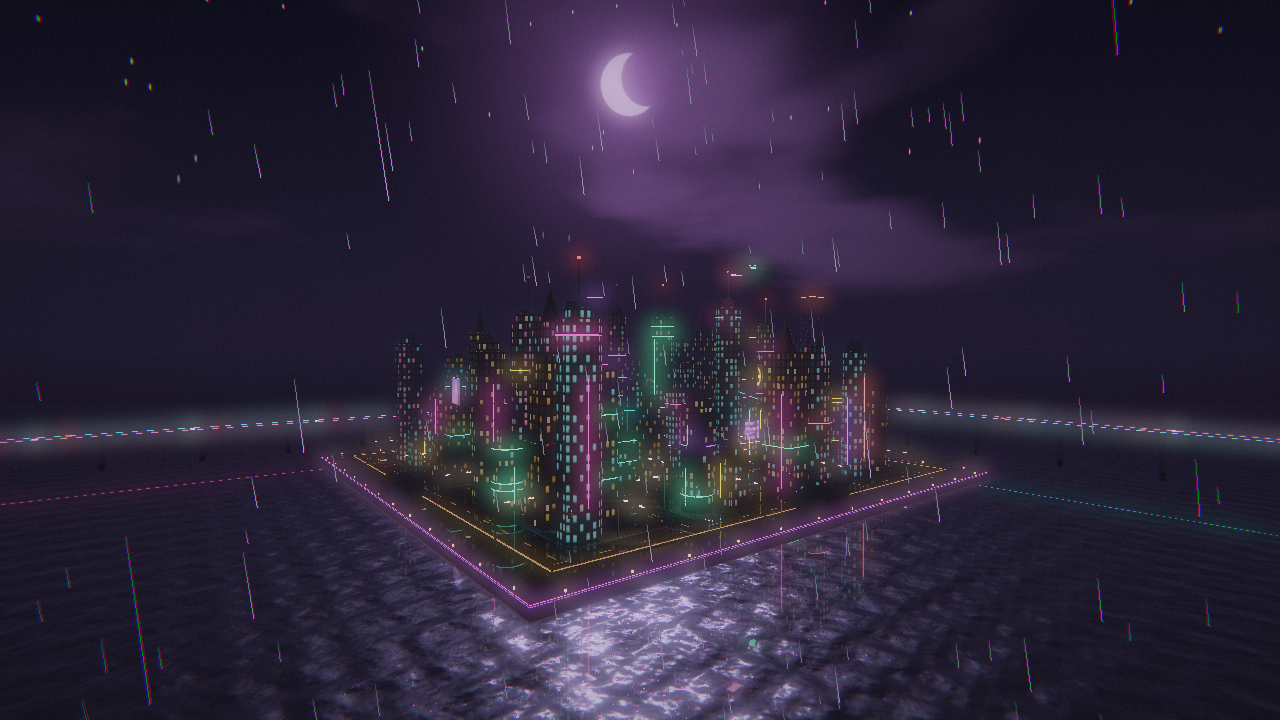
\includegraphics[width=\linewidth]{figures/f01_moon.png}\\{\small (a) Night}
  \end{minipage}\hspace{0.03\textwidth}
  \begin{minipage}{0.40\textwidth}\centering
    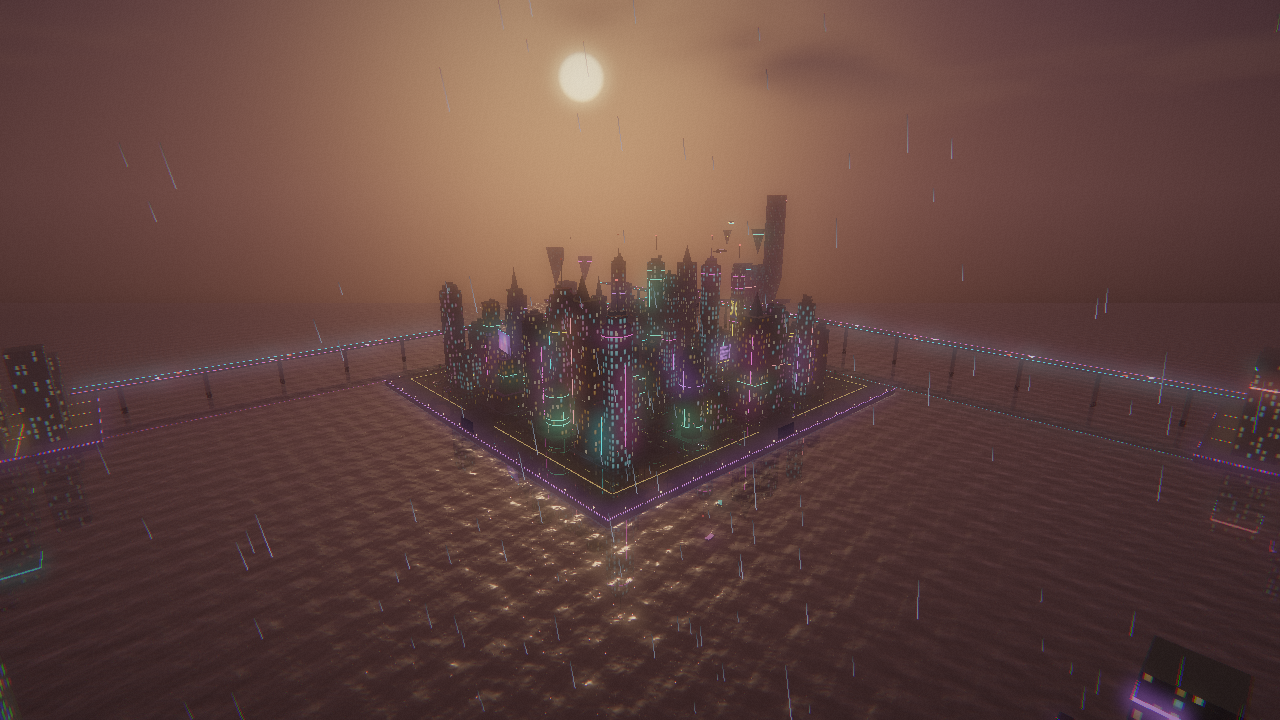
\includegraphics[width=\linewidth]{figures/f02_dusk.png}\\{\small (b) Dusk}
  \end{minipage}\\[4pt]
  \begin{minipage}{0.40\textwidth}\centering
    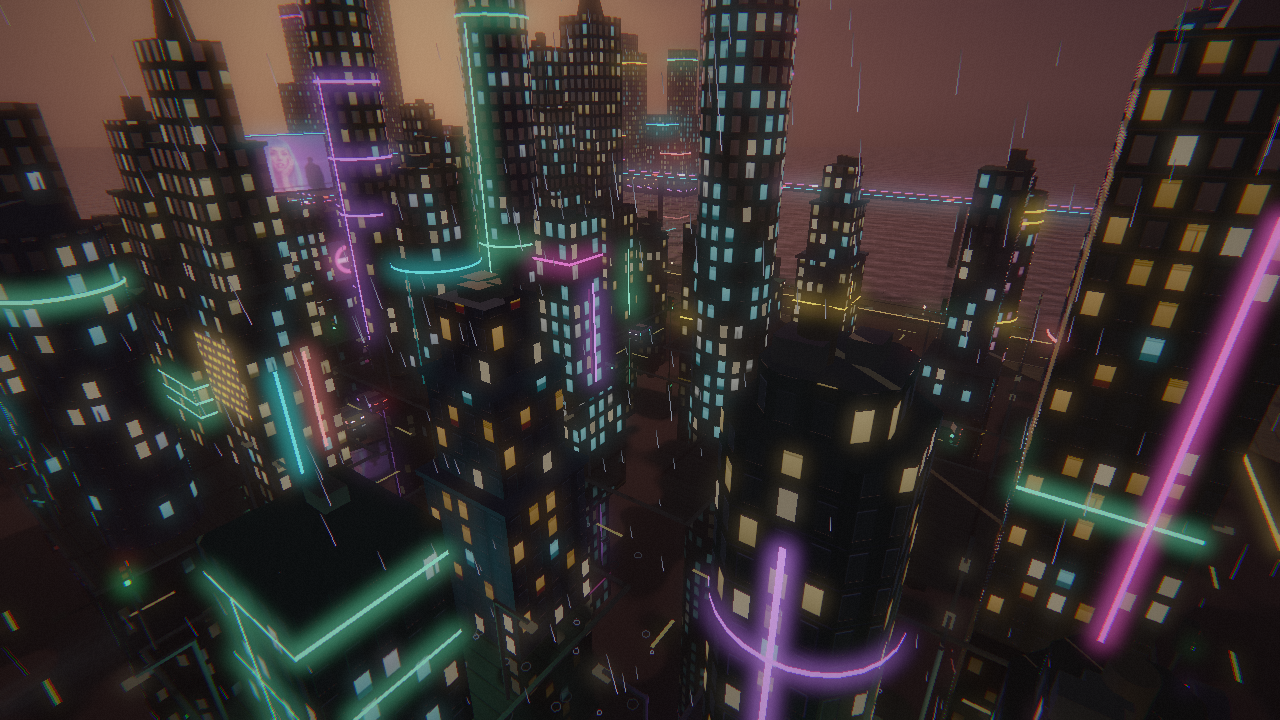
\includegraphics[width=\linewidth]{figures/f03_rt_on.png}\\{\small (c) Ray-traced shadows on}
  \end{minipage}\hspace{0.03\textwidth}
  \begin{minipage}{0.40\textwidth}\centering
    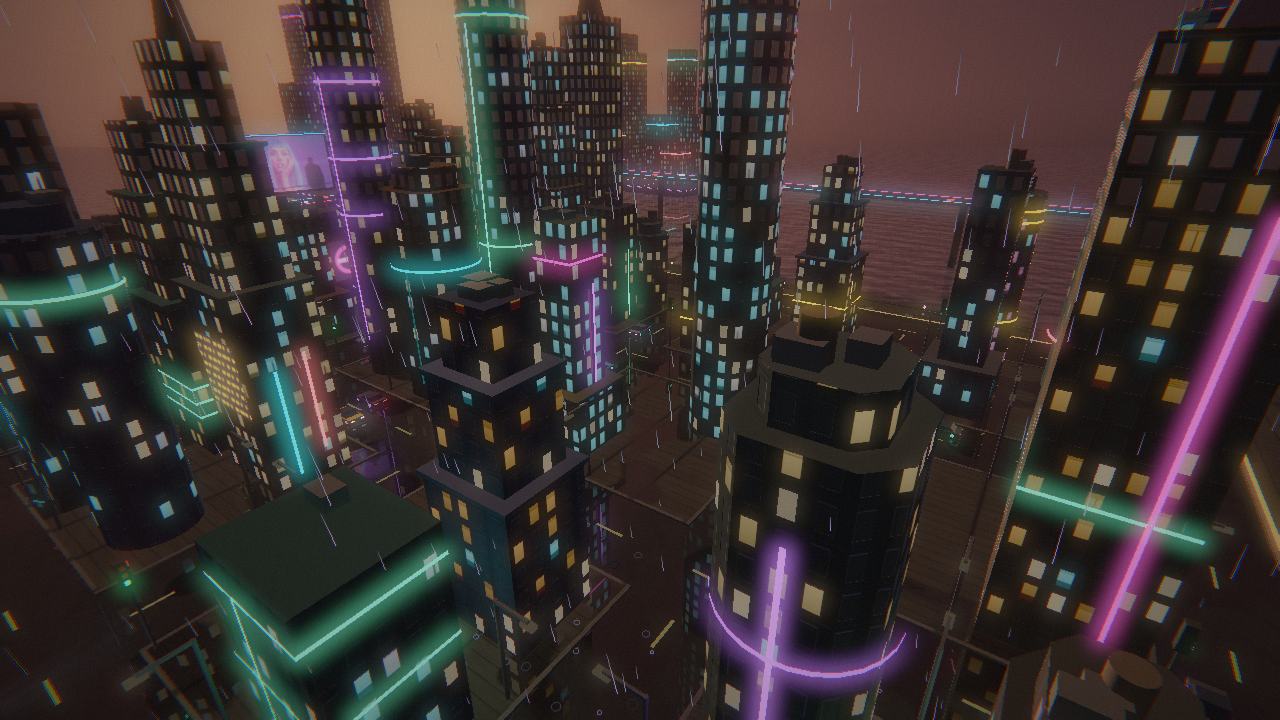
\includegraphics[width=\linewidth]{figures/f04_rt_off.png}\\{\small (d) Shadows off (key H)}
  \end{minipage}
  \caption{The island city and ray-traced sun shadows.}
  \label{fig:4.1}
\end{figure}

\begin{figure}[!htbp]
  \centering
  \begin{minipage}{0.325\textwidth}\centering
    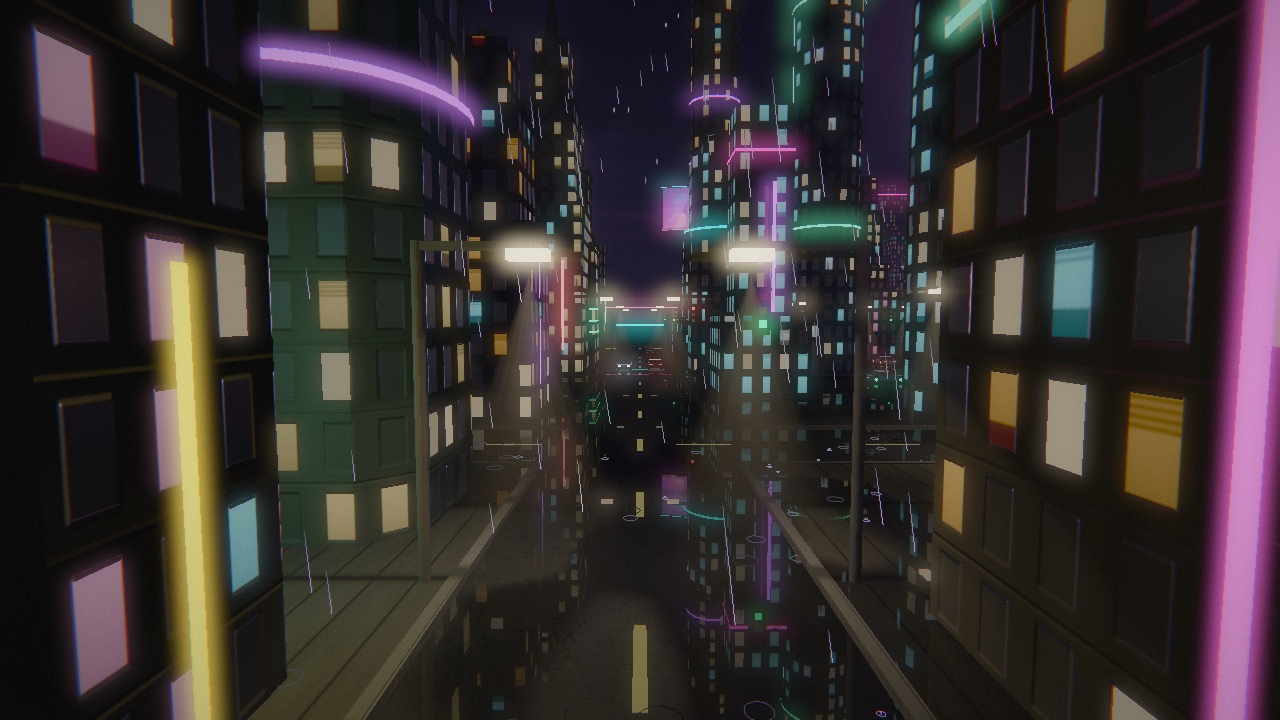
\includegraphics[width=\linewidth]{figures/f05_flat.png}\\{\small (a) Flat}
  \end{minipage}\hfill
  \begin{minipage}{0.325\textwidth}\centering
    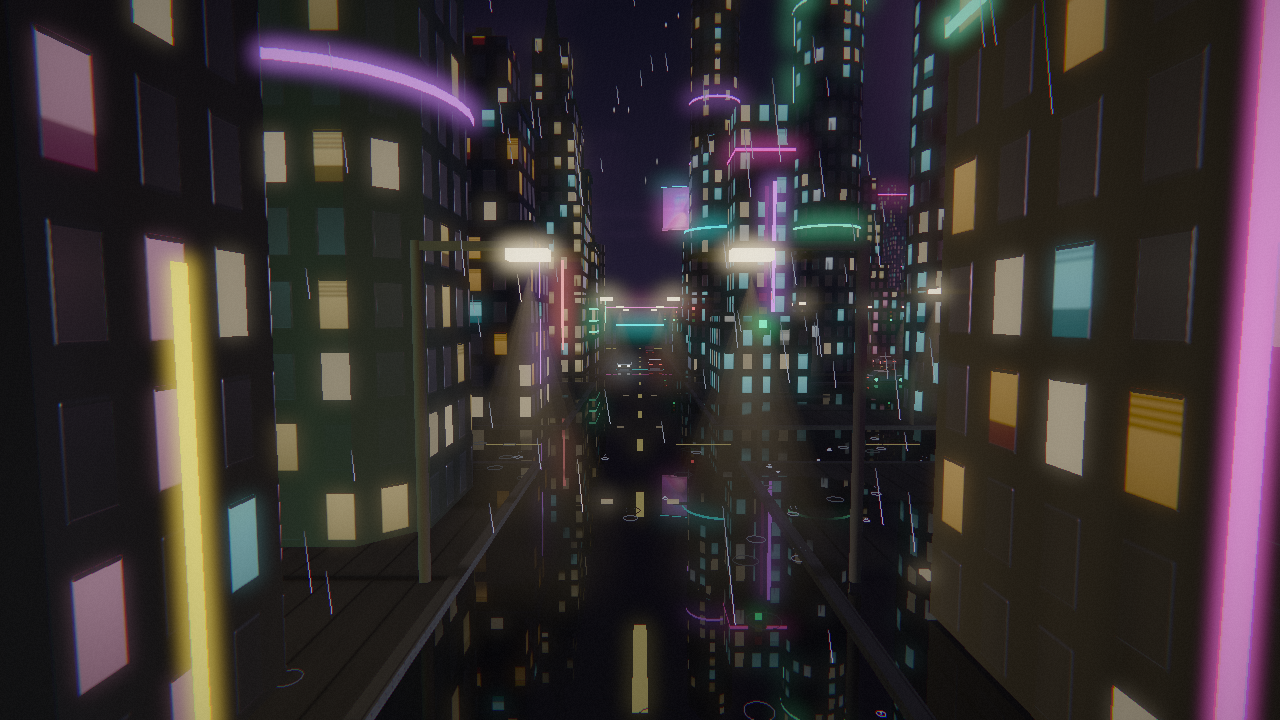
\includegraphics[width=\linewidth]{figures/f06_gouraud.png}\\{\small (b) Gouraud}
  \end{minipage}\hfill
  \begin{minipage}{0.325\textwidth}\centering
    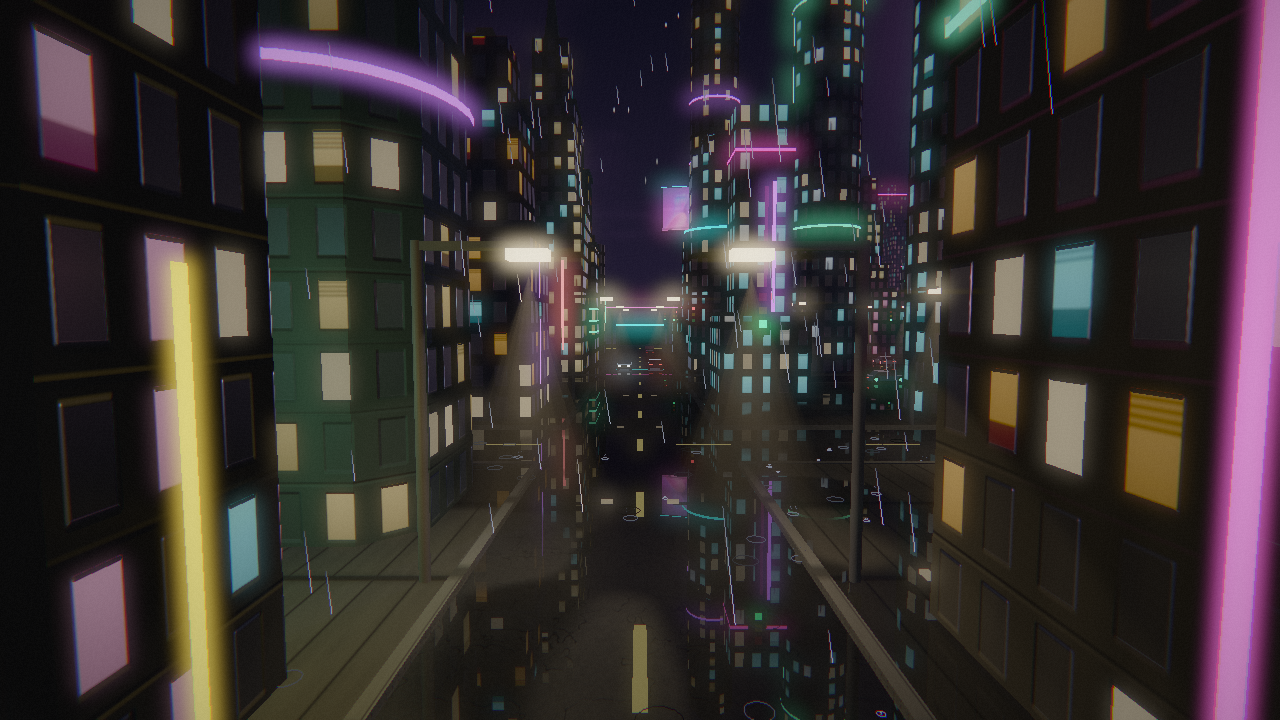
\includegraphics[width=\linewidth]{figures/f07_phong.png}\\{\small (c) Phong}
  \end{minipage}
  \caption{The three shading modes (keys 1--3).}
  \label{fig:4.2}
\end{figure}

\begin{figure}[!htbp]
  \centering
  \begin{minipage}{0.325\textwidth}\centering
    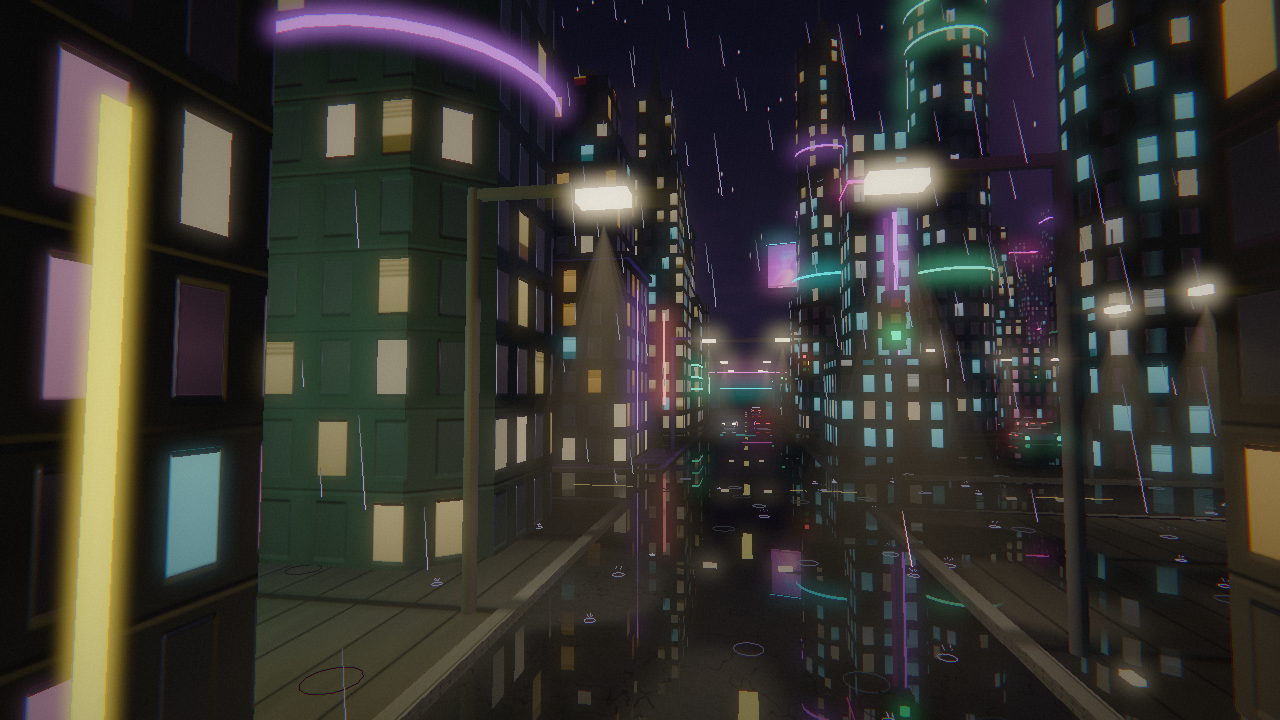
\includegraphics[width=\linewidth]{figures/f08_street.png}\\{\small (a) Spotlights, wet road}
  \end{minipage}\hfill
  \begin{minipage}{0.325\textwidth}\centering
    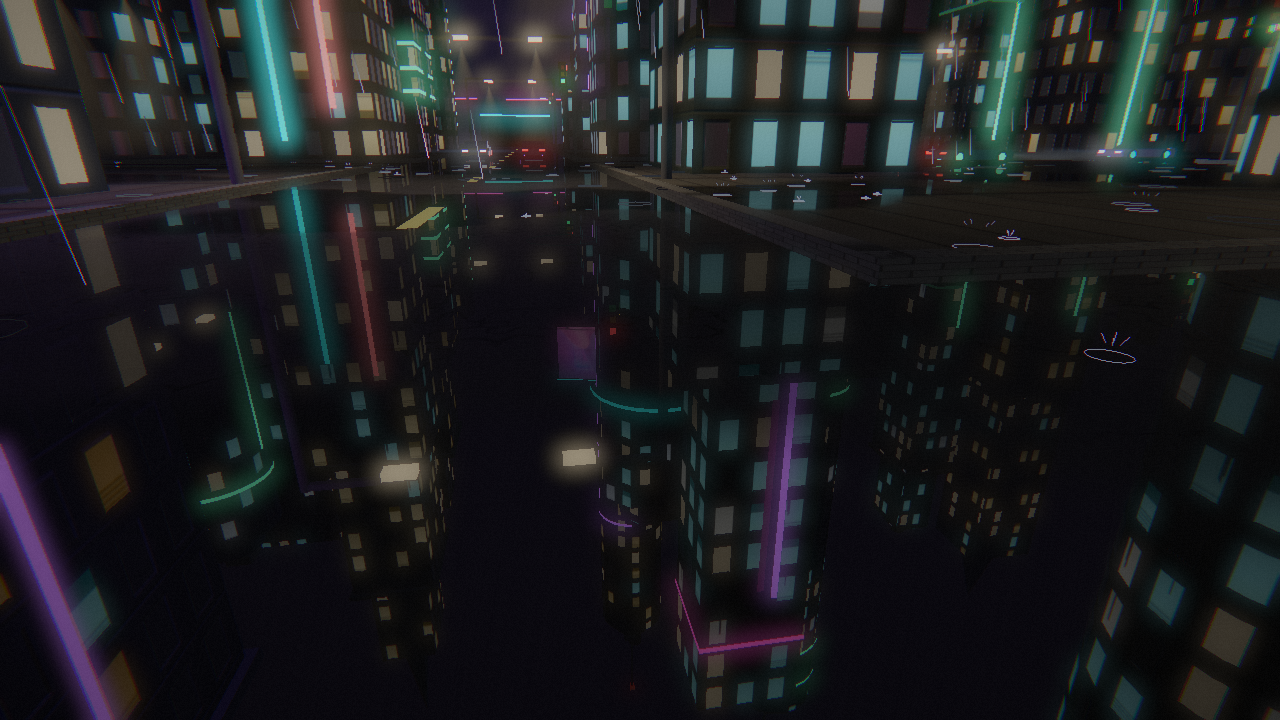
\includegraphics[width=\linewidth]{figures/f14_rain.png}\\{\small (b) Rain and ripples}
  \end{minipage}\hfill
  \begin{minipage}{0.325\textwidth}\centering
    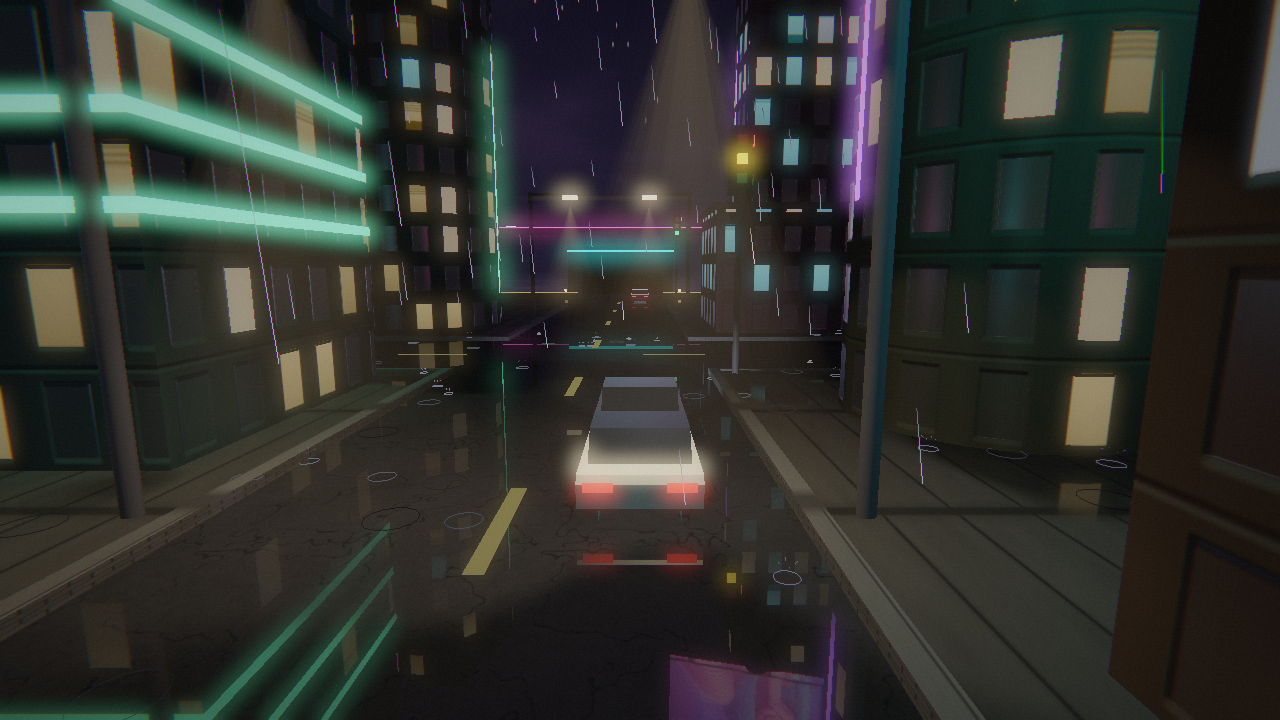
\includegraphics[width=\linewidth]{figures/f15_drive.png}\\{\small (c) Driving}
  \end{minipage}\\[4pt]
  \begin{minipage}{0.325\textwidth}\centering
    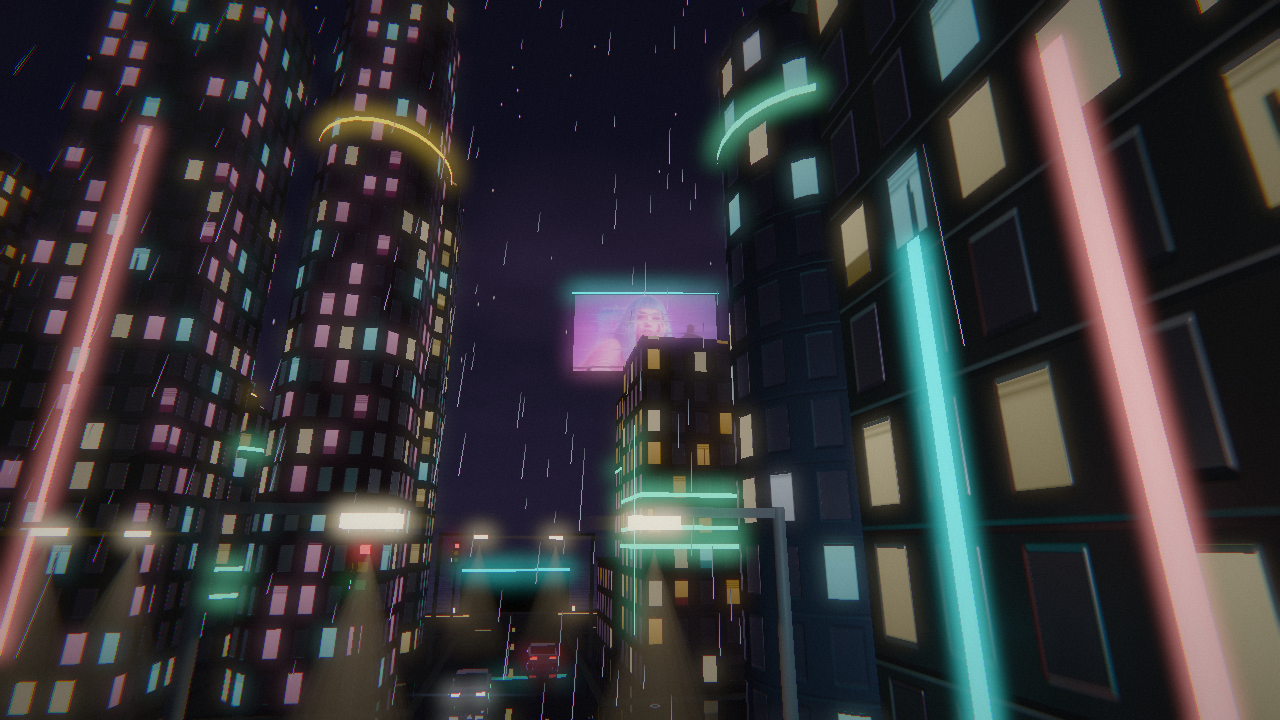
\includegraphics[width=\linewidth]{figures/f09_billboard.png}\\{\small (d) Image billboard}
  \end{minipage}\hfill
  \begin{minipage}{0.325\textwidth}\centering
    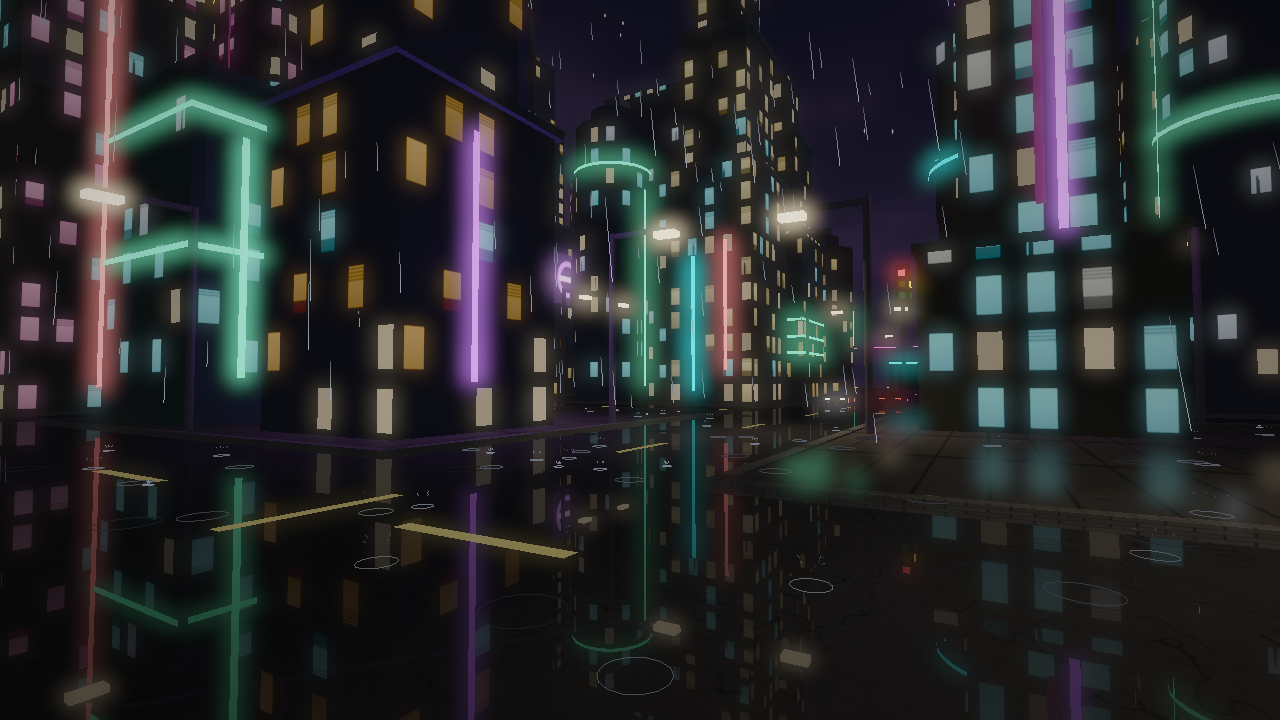
\includegraphics[width=\linewidth]{figures/f17_fx_off.png}\\{\small (e) Detail layer off}
  \end{minipage}\hfill
  \begin{minipage}{0.325\textwidth}\centering
    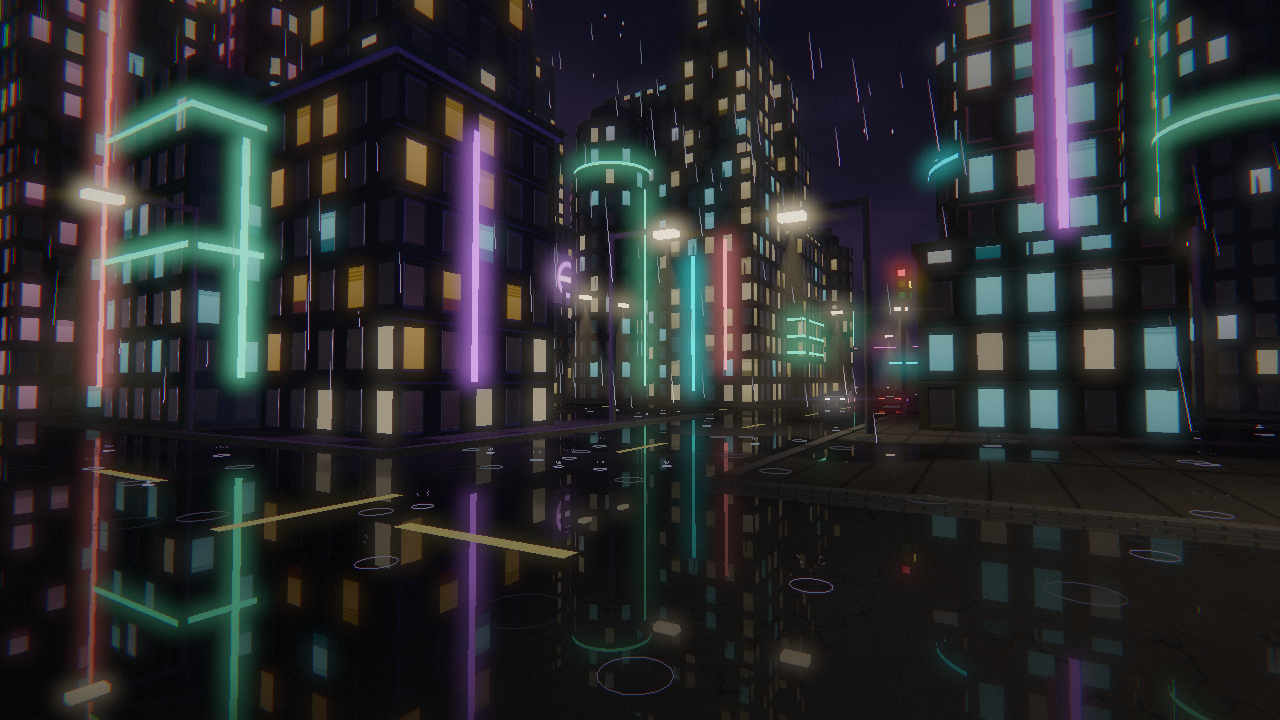
\includegraphics[width=\linewidth]{figures/f18_fx_on.png}\\{\small (f) Detail layer on (X)}
  \end{minipage}
  \caption{Street level, rain, driving, emissive content and the detail layer.}
  \label{fig:4.3}
\end{figure}

\subsection{Quantitative Results}

\begin{table}[!htbp]
  \caption{Scene Statistics, Performance and Verification}
  \label{tab:4.2}
  \centering
  {\fontsize{10}{13}\selectfont
    \begin{tabular}{|p{2.6in}|p{2.7in}|}
      \hline
      \textbf{Metric / test} & \textbf{Value / result} \\
      \hline
      Buildings, parts, neon elements & 53, 246, 148 \\
      \hline
      Street lamps, junctions, AI cars, raindrops & 80, 25, 18, 1,500 \\
      \hline
      Source code & 7,131 lines in 10 files \\
      \hline
      FPS, all effects, $1280\times720$ (18 test views) & 77--161 \\
      \hline
      Same view: RT on / off; detail layer off / on & 103 / 109 FPS; 96 / 78 FPS \\
      \hline
      RT shadows on vs off, same view & 14.6\% of pixels darker, 0\% lighter (correct) \\
      \hline
      Traffic, 10 min simulated, 6 seeds & 0 collisions, 0 off road, none stuck \\
      \hline
      Ring-road congestion after tuning & 8--11 of 18 cars $\rightarrow$ 1--7 \\
      \hline
    \end{tabular}
  }
\end{table}

\subsection{Analysis of the Results}

\begin{justify}
  {\fontsize{12}{13.8}\selectfont
    Ray-traced shadows are cheap because the grid limits each ray to a few blocks; the on/off test confirms correctness, since a shadow only removes light. The largest costs were the mirrored pass and bloom, reduced by sending only 8 lights to the reflection and blurring at half resolution; fullscreen is capped at $1440\times810$ and upscaled. Traffic tests caught a congested ring road, fixed by raising its exit chance from 25\% to 60\%.
  }
\end{justify}

\section{Objectives Achieved}

\begin{justify}
  {\fontsize{12}{13.8}\selectfont
    All seven objectives were met. The only proposal item that changed was screen-space reflection, replaced by planar reflection for performance. Table 4.3 links every objective to the feature and the evidence that shows it.
  }
\end{justify}

\begin{table}[!htbp]
  \caption{Objectives and Evidence}
  \label{tab:4.3}
  \centering
  {\fontsize{10}{12.5}\selectfont
    \begin{tabular}{|p{1.7in}|p{2.2in}|p{1.5in}|}
      \hline
      \textbf{Objective} & \textbf{How it was met} & \textbf{Evidence} \\
      \hline
      Reproducible procedural city & LCG seeded with 2107015; key N makes a new seed & Same city every run; Fig. 4.1 \\
      \hline
      Primitives and transformations & Unit meshes placed by $M=TRS$; hierarchical cars, lamps & Section III.2.2--III.2.3 \\
      \hline
      Lighting and shading & 4 light types, Blinn--Phong; flat, Gouraud, Phong on keys 1--3 & Fig. 4.2, Table 3.3 \\
      \hline
      Single-clock animation & Traffic, rain, signals, neon, sunset from one clock; P pauses & Demo video \\
      \hline
      Ray tracing and effects & Shadow rays with grid, reflections, bloom, fog, sky & Fig. 4.1; 14.6\% darker pixels \\
      \hline
      Rich interaction & Flying camera, driving, 20+ toggles, camera tour, pause menu & Table 3.4 \\
      \hline
      Above 60 FPS on iGPU & Light ranking, half-size bloom, dynamic resolution & Table 4.2: 77--161 FPS \\
      \hline
    \end{tabular}
  }
\end{table}

\section{Discussion}

\begin{justify}
  {\fontsize{12}{13.8}\selectfont
    The results show that the course topics combine well in one scene. Lighting and shading are visible everywhere because the city is lit almost only by its own lamps, neon and windows, so switching between flat, Gouraud and Phong changes the image clearly. Ray tracing was the most valuable addition: it needed only a few hundred lines of shader code, yet it gives the dusk scene its depth. The main trade-off was between visual richness and speed. Every expensive effect (reflection, bloom, detail layer) was made cheaper or switchable, so the program stays interactive on a laptop with integrated graphics and every effect can be shown on and off during a demonstration.
  }
\end{justify}

\subsection*{Cost of the Shading Modes}

\begin{justify}
  {\fontsize{12}{13.8}\selectfont
    Table 4.4 compares the frame rate of the three shading modes and of two switchable features from the same camera view, measured with the built-in screenshot mode at $1280\times720$ with vsync off.
  }
\end{justify}

\begin{table}[!htbp]
  \caption{Frame Rate by Shading Mode and Feature (same view, $1280\times720$)}
  \label{tab:4.4}
  \centering
  {\fontsize{10}{12.5}\selectfont
    \begin{tabular}{|p{2.2in}|p{0.9in}|p{2.3in}|}
      \hline
      \textbf{Setting} & \textbf{FPS} & \textbf{Reason} \\
      \hline
      Flat shading (key 1) & 82--83 & per-pixel lighting with one face normal \\
      \hline
      Gouraud shading (key 2) & 113--117 & lighting only at vertices; no shadow rays \\
      \hline
      Phong shading (key 3) & 76--77 & full lighting and shadow rays per pixel \\
      \hline
      Ray-traced shadows on / off (key H) & 103 / 105--113 & one shadow ray per lit pixel \\
      \hline
      Detail layer off / on (key X) & 95--97 / 73--79 & bump mapping, puddles, beams, lens effects \\
      \hline
    \end{tabular}
  }
\end{table}

\begin{justify}
  {\fontsize{12}{13.8}\selectfont
    Gouraud is the fastest because the lighting loop runs once per vertex instead of once per pixel, and a building wall has only a few vertices but thousands of pixels. Its cost is visible in Figure 4.2: lamp light that falls inside a large triangle is lost. Phong is the slowest but most accurate and is therefore the default; the difference stays small because the light count is capped at 24.
  }
\end{justify}

\section{Conclusion}

\begin{justify}
  {\fontsize{12}{13.8}\selectfont
    Every proposed feature was delivered, one was replaced by a faster equivalent, and ray tracing and several further systems were added. The screenshots confirm that each lighting, shading and ray-tracing feature works as intended, and the measurements show the program stays well above 60 FPS on integrated graphics. The traffic and ray-tracing tests also give evidence of correctness that does not depend on judging the image by eye.
  }
\end{justify}

%==============================================================
% CHAPTER V: Impact Analysis
%==============================================================
\chapter{Societal, Health, Environment, Safety, Ethical, Legal and Cultural Issues}

\section{Intellectual Property and Legal Considerations}

\begin{justify}
  {\fontsize{12}{13.8}\selectfont
    The libraries used are open source with permissive licences: GLFW (zlib/libpng licence), GLAD (MIT) and GLM (MIT). They allow use and redistribution in academic and commercial work as long as their copyright notices are kept. All 3D geometry and almost every texture are generated by the program's own code, so the project contains no third-party models or artwork. The only exceptions are the background music tracks and the picture on the rooftop billboards, which are copyrighted works used here only for a non-commercial classroom demonstration. A public release would replace them with royalty-free or licensed material, and the music can already be switched off with key M. The visual style is inspired by cyberpunk films and games, but no assets, names or logos from them are used.
  }
\end{justify}

\section{Ethical, Safety and Health Considerations}

\begin{justify}
  {\fontsize{12}{13.8}\selectfont
    The application collects no personal data and needs no network connection. Flickering lights can trouble photosensitive viewers, so flicker is limited to a few slow neon signs, and the whole animation stops with key P or the pause menu. To avoid motion sickness the flying speed is moderate and the chase camera and camera tour move smoothly. Music volume is low by default, and vsync stops the laptop running hot during long sessions.
  }
\end{justify}

\section{Impact on Societal, Cultural and Environmental Issues}

\begin{justify}
  {\fontsize{12}{13.8}\selectfont
    Many students in Bangladesh use laptops with integrated graphics rather than expensive dedicated GPUs. Showing that ray-traced shadows, reflections and bloom can run in real time on such hardware makes advanced graphics more accessible for learning. Because every effect can be switched on and off, the program also works as a teaching tool: a teacher can show the same scene with and without Gouraud shading, shadows or reflections. On the environmental side, the efficiency measures (choosing only 24 lights, blurring at half resolution, dynamic resolution and vsync) reduce the power the GPU uses, which matters for battery life and energy use. Culturally, the project uses a neutral, fictional city and does not depict real people, places or groups.
  }
\end{justify}

%==============================================================
% CHAPTER VI: Complex Engineering Problems and Activities
%==============================================================
\chapter{Addressing Complex Engineering Problems and Activities}

\section{Complex Engineering Problems Associated with the Current Project}

\begin{table}[!htbp]
  \caption{Complex Engineering Problems}
  \label{tab:6.1}
  \centering
  {\fontsize{10}{13}\selectfont
    \begin{tabular}{|p{1.3in}|p{2.1in}|p{2.0in}|}
      \hline
      \textbf{Problem} & \textbf{Challenge} & \textbf{Solution} \\
      \hline
      Many lights & 200+ lights, fixed shader budget & Score and keep the best 24 each frame \\
      \hline
      Ray tracing cost & One ray per pixel against 127 boxes & Uniform grid, DDA traversal, early exit \\
      \hline
      Reflection correctness & Mirror flips winding and leaks geometry & Flip front face; clip plane \\
      \hline
      Traffic safety & Cars overlapping at junctions and turns & Lanes, following gap, signal and junction-box rules; tested over 10 min \\
      \hline
      Performance & 1080p and second geometry pass on iGPU & Render scale, half-res bloom, fewer lights in reflection \\
      \hline
      Effect balance & Streaks on every neon; mirror-like streets & Streak mask in the bright image's alpha; dimmed reflection pass \\
      \hline
    \end{tabular}
  }
\end{table}

\section{Complex Engineering Activities Associated with the Current Project}

\begin{justify}
  {\fontsize{12}{13.8}\selectfont
    The project combined linear algebra, physics-inspired models (attenuation, Fresnel, braking distance) and algorithms (ray--box tests, grid traversal, partial sorting), verified by headless traffic tests and repeatable screenshot comparisons. Table 6.2 describes these activities against the usual attributes of complex engineering activities.
  }
\end{justify}

\begin{table}[!htbp]
  \caption{Complex Engineering Activities}
  \label{tab:6.2}
  \centering
  {\fontsize{10}{13}\selectfont
    \begin{tabular}{|p{1.4in}|p{4.0in}|}
      \hline
      \textbf{Attribute} & \textbf{In this project} \\
      \hline
      Range of resources & GPU time, memory and a fixed light budget had to be shared between lighting, ray tracing, reflection and post-processing \\
      \hline
      Level of interaction & Lighting, shadows, reflection, traffic and the time of day all affect each other; for example the sun's light depends on dusk, the shadows depend on the sun, and the lamps switch on as it sets \\
      \hline
      Innovation & Shader-based ray tracing with a grid on an integrated GPU, and an importance score to choose lights every frame \\
      \hline
      Consequences & Wrong settings make the scene unreadable (too dark, too bright, mirror-like streets) or too slow, so each change was measured with repeatable screenshots and FPS logs \\
      \hline
      Familiarity & Most techniques (ray tracing, Fresnel, bloom, traffic simulation) went beyond the laboratory work and were learned from papers and tutorials \\
      \hline
    \end{tabular}
  }
\end{table}

%==============================================================
% CHAPTER VII: Conclusions
%==============================================================
\chapter{Conclusions}

\section{Summary}

\begin{justify}
  {\fontsize{12}{13.8}\selectfont
    Neon Genesis renders a procedural, animated cyberpunk city in real time with four light types, three shading modes, ray-traced shadows, reflections, bloom, a detail layer of surface and lens effects, AI traffic and a drivable car, above 60 FPS on integrated graphics.
  }
\end{justify}
\begin{justify}
  {\fontsize{12}{13.8}\selectfont
    The project met all of the course requirements: lighting with ambient, directional, point and spot lights; transformations including hierarchical models; Gouraud and Phong shading (with flat shading for comparison); continuous motion and animation; and interaction through the keyboard, the mouse, a drivable car and a pause menu. Ray-traced shadows were added for the bonus. Building it showed how much a real-time scene depends on careful budgeting: the same few ideas (unit shapes placed by matrices, one lighting function and one clock) were reused everywhere, which kept the code understandable while the scene grew.
  }
\end{justify}

\section{Limitations}

\begin{justify}
  {\fontsize{12}{13.8}\selectfont
    \begin{itemize}\setlength{\itemsep}{0pt}\setlength{\parskip}{0pt}
      \item Shadows are hard-edged; only the sun and moon cast them, and round towers cast box-shaped shadows.
      \item Cars only turn right and do not cast shadows; car reflections use a faked environment, not the real city.
      \item The reflection is planar, so only flat surfaces (road, water) reflect, and it is slightly offset on the water.
      \item Only 24 lights are used per pixel, so far-away lamps do not light the surfaces near them.
      \item Audio, image loading and the pause menu depend on Windows APIs, so the program runs only on Windows.
    \end{itemize}
  }
\end{justify}

\section{Recommendations and Future Works}

\begin{justify}
  {\fontsize{12}{13.8}\selectfont
    Several extensions would make the project more complete:
    \begin{itemize}\setlength{\itemsep}{0pt}\setlength{\parskip}{0pt}
      \item \textbf{Soft shadows:} several jittered shadow rays per pixel for a soft penumbra.
      \item \textbf{More ray tracing:} lamp shadows and reflections on curved car bodies.
      \item \textbf{Clustered lighting:} let every lamp light the scene, not only the best 24.
      \item \textbf{Smarter traffic:} left turns, lane changes and pedestrians.
      \item \textbf{Cross-platform build:} portable audio and image libraries.
    \end{itemize}
  }
\end{justify}

%==============================================================
% REFERENCES
%==============================================================
\clearpage
\addcontentsline{toc}{chapter}{References}

\begin{center}
  {\fontsize{14}{21}\bfseries REFERENCES}
\end{center}

\begin{spacing}{1.0}
  \begin{list}{}{
    \setlength{\leftmargin}{0.31in}
    \setlength{\itemindent}{-0.31in}
    \setlength{\topsep}{0pt}
    \setlength{\itemsep}{2pt}
    \setlength{\parsep}{0pt}
  }
    \fontsize{10}{12}\selectfont

    \item[1.] Khronos Group, ``The OpenGL Graphics System: A Specification, Version 3.3 (Core Profile),'' 2010.

    \item[2.] GLFW Development Team, ``GLFW Documentation,'' [Online]. Available: https://www.glfw.org/docs/latest/.

    \item[3.] G-Truc Creation, ``OpenGL Mathematics (GLM),'' [Online]. Available: https://github.com/g-truc/glm.

    \item[4.] J. de Vries, \textit{Learn OpenGL: Learn Modern OpenGL Graphics Programming}, 2020. [Online]. Available: https://learnopengl.com/.

    \item[5.] B. T. Phong, ``Illumination for Computer Generated Pictures,'' \textit{Communications of the ACM}, vol. 18, no. 6, pp. 311--317, 1975.

    \item[6.] J. F. Blinn, ``Models of Light Reflection for Computer Synthesized Pictures,'' in \textit{Proc. SIGGRAPH}, 1977, pp. 192--198.

    \item[7.] H. Gouraud, ``Continuous Shading of Curved Surfaces,'' \textit{IEEE Trans. Computers}, vol. C-20, no. 6, pp. 623--629, 1971.

    \item[8.] T. Whitted, ``An Improved Illumination Model for Shaded Display,'' \textit{Communications of the ACM}, vol. 23, no. 6, pp. 343--349, 1980.

    \item[9.] T. L. Kay and J. T. Kajiya, ``Ray Tracing Complex Scenes,'' in \textit{Proc. SIGGRAPH}, 1986, pp. 269--278.

    \item[10.] J. Amanatides and A. Woo, ``A Fast Voxel Traversal Algorithm for Ray Tracing,'' in \textit{Proc. Eurographics}, 1987, pp. 3--10.

    \item[11.] E. Reinhard, M. Stark, P. Shirley, and J. Ferwerda, ``Photographic Tone Reproduction for Digital Images,'' \textit{ACM Trans. Graphics}, vol. 21, no. 3, pp. 267--276, 2002.

    \item[12.] C. Schlick, ``An Inexpensive BRDF Model for Physically-Based Rendering,'' \textit{Computer Graphics Forum}, vol. 13, no. 3, pp. 233--246, 1994.

    \item[13.] E. Catmull and R. Rom, ``A Class of Local Interpolating Splines,'' in \textit{Computer Aided Geometric Design}, Academic Press, 1974, pp. 317--326.

    \item[14.] K. Perlin, ``An Image Synthesizer,'' in \textit{Proc. SIGGRAPH}, 1985, pp. 287--296.

    \item[15.] W. H. Press, S. A. Teukolsky, W. T. Vetterling, and B. P. Flannery, \textit{Numerical Recipes}, 3rd ed., Cambridge University Press, 2007.

    \item[16.] D. Hearn, M. P. Baker, and W. Carithers, \textit{Computer Graphics with OpenGL}, 4th ed., Pearson, 2011.

    \item[17.] J. F. Blinn, ``Simulation of Wrinkled Surfaces,'' in \textit{Proc. SIGGRAPH}, 1978, pp. 286--292.

    \item[18.] Y. I. H. Parish and P. M\"uller, ``Procedural Modeling of Cities,'' in \textit{Proc. SIGGRAPH}, 2001, pp. 301--308.

    \item[19.] KUET CSE Computer Graphics Laboratory, starter code (GLFW + GLAD + GLM triangle and rectangle), 2026.

  \end{list}
\end{spacing}

\end{document}
